\documentclass[12pt]{article}
\usepackage{amsmath, amssymb, amsthm}
\usepackage{bm}
\usepackage{geometry}
\usepackage{hyperref}
\usepackage{graphicx}
\usepackage{booktabs}
\usepackage{array}
\usepackage{multirow}
\usepackage{float}
\usepackage{tabularx}
\usepackage{ragged2e}
\usepackage{xcolor}
\usepackage{listings}
\usepackage{graphicx}
\usepackage{algorithm}
\usepackage{algpseudocode}

\geometry{margin=1in}

% Theorem environments
\newtheorem{theorem}{Theorem}
\newtheorem{lemma}[theorem]{Lemma}
\newtheorem{proposition}[theorem]{Proposition}
\newtheorem{corollary}[theorem]{Corollary}
\newtheorem{definition}{Definition}
\newtheorem{remark}{Remark}
\newtheorem{example}{Example}

% Custom commands
\newcommand{\R}{\mathbb{R}}
\newcommand{\E}{\mathbb{E}}
\newcommand{\Var}{\text{Var}}
\newcommand{\Cov}{\text{Cov}}
\newcommand{\tr}{\text{tr}}
\newcommand{\diag}{\text{diag}}
\DeclareMathOperator*{\argmin}{arg\,min}
\DeclareMathOperator*{\argmax}{arg\,max}

% Code listing settings
\lstset{
    language=R,
    basicstyle=\small\ttfamily,
    breaklines=true,
    frame=single,
    numbers=left,
    numberstyle=\tiny,
    captionpos=b
}



\begin{document}
\begin{titlepage}
 \centering % Center everything on the page
 
 \vspace*{1cm} % Add some space at the top
 
 {\Huge \bfseries Splines and Smoothing: Complete Mathematical Derivations with GAM Applications}
 
 \vspace{2cm} % Space between title and image
 
 % --- IMAGE ---
 % Make sure the image file 'spline-ducks.png' is in the same directory
 % as your .tex file. Adjust width as needed.
 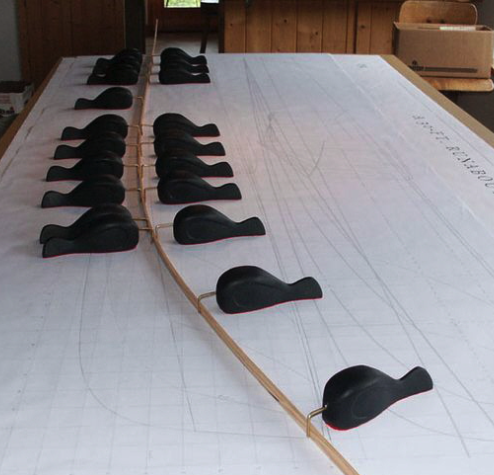
\includegraphics[width=0.6\linewidth]{spline-ducks.png}
 
 \vfill % Pushes the content below to the bottom of the page
  
 \vspace{1cm}
 
 {\large \today}

\end{titlepage}
\maketitle
\tableofcontents
\newpage

%% PART I: FOUNDATIONS %%
\part{Foundations and Motivation}

\section{Introduction: The Physical Analogy and Statistical Motivation}

\subsection{The Draftsman's Spline}

The term ``spline'' originates from a flexible wooden strip used by draftsmen. When bent against fixed points (lead weights or ``ducks''), the strip naturally assumes a shape that minimizes its total bending energy. This physical principle provides profound insight into the mathematical framework of spline smoothing.

\begin{definition}[Bending Energy]
For a function $f: [a,b] \to \R$ with continuous second derivative, the bending energy is:
\begin{equation}
E[f] = \int_a^b [f''(x)]^2 \, dx
\end{equation}
\end{definition}

This energy minimization principle directly translates to our statistical goal: finding a smooth function that balances fidelity to observed data with smoothness constraints.

\subsection{The Fundamental Trade-off in GAMs}

In the context of Generalized Additive Models (GAMs), we face a central challenge in nonparametric regression:

\begin{itemize}
    \item \textbf{Fidelity to data}: We want our fitted function to pass close to the observed data points, minimizing $\sum_{i=1}^n (y_i - f(x_i))^2$
    \item \textbf{Smoothness}: We want to avoid overfitting by controlling the roughness of $f$, typically measured by $\int [f''(x)]^2 dx$
\end{itemize}

\begin{example}[Why smoothness matters]
Consider fitting a function to noisy data. Without any smoothness constraint, we could interpolate exactly through every data point, but this would likely capture noise rather than the underlying signal. The smoothness penalty acts as a regularizer, encouraging the fitted function to vary slowly except where the data strongly suggest otherwise.
\end{example}

This trade-off is formalized in the penalized likelihood framework that underlies modern GAM fitting.

%% PART II: BASIS FUNCTIONS %%
\part{From Basis Functions to Penalized Splines}
\begin{figure}[h!]
 \centering
 \includegraphics[width=\linewidth]{b-splines.png}
 \caption{B Spline Basis Functions}
 \label{fig:enter-label-1}
\end{figure}
\section{Basis Function Representations}

\subsection{The Basis Expansion Framework}

The key insight that makes spline smoothing computationally tractable is representing smooth functions as linear combinations of basis functions.

\begin{definition}[Basis Expansion]
A function $f: \R \to \R$ is represented as a linear combination of basis functions:
\begin{equation}
f(x) = \sum_{k=1}^{K} \beta_k b_k(x)
\end{equation}
where $\{b_k(x)\}_{k=1}^K$ are known basis functions and $\{\beta_k\}_{k=1}^K$ are coefficients to be estimated.
\end{definition}

\textbf{Intuition for GAMs:} This representation transforms the infinite-dimensional problem of estimating a function into a finite-dimensional problem of estimating $K$ coefficients. The choice of basis functions determines the flexibility and computational properties of the resulting smoother.

\subsection{Truncated Power Basis}

The truncated power basis provides a direct construction of piecewise polynomials.

\begin{definition}[Truncated Power Function]
For a knot $\kappa$ and degree $d$, the truncated power function is:
\begin{equation}
(x - \kappa)_+^d = \begin{cases}
(x - \kappa)^d & \text{if } x > \kappa \\
0 & \text{if } x \leq \kappa
\end{cases}
\end{equation}
\end{definition}

For a spline of degree $d$ with knots $\kappa_1, \ldots, \kappa_M$, the basis consists of:
\begin{align}
\{1, x, x^2, \ldots, x^d, (x-\kappa_1)_+^d, (x-\kappa_2)_+^d, \ldots, (x-\kappa_M)_+^d\}
\end{align}

\textbf{GAM Context:} While conceptually simple, truncated power bases can be numerically unstable for large $d$ or many knots. This motivates the use of B-splines in practice.

\subsection{B-splines: The Computational Workhorse}

B-splines are the preferred basis for most GAM implementations due to their excellent numerical properties.

\begin{definition}[B-spline Recursion]
For degree $d$ and knot sequence $\{t_i\}$:
\begin{align}
B_{i,0}(x) &= \begin{cases}
1 & \text{if } t_i \leq x < t_{i+1} \\
0 & \text{otherwise}
\end{cases} \\
B_{i,d}(x) &= \frac{x - t_i}{t_{i+d} - t_i} B_{i,d-1}(x) + \frac{t_{i+d+1} - x}{t_{i+d+1} - t_{i+1}} B_{i+1,d-1}(x)
\end{align}
\end{definition}

\textbf{Key Properties for GAMs:}
\begin{itemize}
    \item \textbf{Local support}: Each B-spline is non-zero only over $d+2$ adjacent knot intervals
    \item \textbf{Partition of unity}: $\sum_i B_{i,d}(x) = 1$ for all $x$
    \item \textbf{Numerical stability}: Well-conditioned even for high degrees
    \item \textbf{Efficient computation}: Sparse model matrices due to local support
\end{itemize}

\subsection{The Model Matrix}

\begin{definition}[Model Matrix]
Given observations $(x_i, y_i)_{i=1}^n$ and basis functions $\{b_k\}_{k=1}^K$, the model matrix $\mathbf{X} \in \R^{n \times K}$ has entries:
\begin{equation}
X_{ik} = b_k(x_i)
\end{equation}
\end{definition}

This transforms the function estimation problem into the familiar linear model framework:
\begin{equation}
\mathbf{y} = \mathbf{X}\bm{\beta} + \bm{\epsilon}
\end{equation}

\textbf{GAM Insight:} The model matrix encodes how each basis function contributes to the predictions at each data point. For B-splines, this matrix is sparse, enabling efficient computation even with many basis functions.

%% PART III: PENALIZED SPLINES %%
\part{The Penalized Spline Solution}

\section{Penalized Regression Splines}

\subsection{The Penalized Objective Function}

The key innovation in modern GAM fitting is the use of penalized estimation, which elegantly balances fit and smoothness.

\begin{definition}[Penalized Least Squares]
The penalized least squares objective is:
\begin{equation}
\mathcal{L}(\bm{\beta}) = \|\mathbf{y} - \mathbf{X}\bm{\beta}\|^2 + \lambda \bm{\beta}^T \mathbf{S} \bm{\beta}
\end{equation}
where:
\begin{itemize}
    \item $\lambda \geq 0$ is the smoothing parameter
    \item $\mathbf{S}$ is the penalty matrix
\end{itemize}
\end{definition}

\textbf{Interpretation in GAMs:}
\begin{itemize}
    \item The first term measures goodness-of-fit (data fidelity)
    \item The second term measures roughness (complexity) of the fitted function
    \item $\lambda$ controls the trade-off: large $\lambda$ gives smoother fits, small $\lambda$ gives more flexible fits
    \item The penalty matrix $\mathbf{S}$ encodes what we mean by "roughness"
\end{itemize}

\section{Constructing Penalty Matrices}

\subsection{Derivative-based Penalties}

The most natural measure of function roughness is based on derivatives.

\begin{theorem}[Derivative Penalty in Basis Form]
For the functional penalty $J_m(f) = \int [f^{(m)}(x)]^2 dx$ and basis expansion $f(x) = \sum_{k=1}^K \beta_k b_k(x)$:
\begin{equation}
J_m(f) = \bm{\beta}^T \mathbf{S} \bm{\beta}
\end{equation}
where $S_{jk} = \int b_j^{(m)}(x) b_k^{(m)}(x) dx$.
\end{theorem}

\begin{proof}
Starting with $f(x) = \sum_{k=1}^K \beta_k b_k(x)$, the $m$-th derivative is:
\begin{equation}
f^{(m)}(x) = \sum_{k=1}^K \beta_k b_k^{(m)}(x)
\end{equation}

Therefore:
\begin{align}
J_m(f) &= \int \left[f^{(m)}(x)\right]^2 dx \\
&= \int \left[\sum_{j=1}^K \beta_j b_j^{(m)}(x)\right] \left[\sum_{k=1}^K \beta_k b_k^{(m)}(x)\right] dx \\
&= \int \sum_{j=1}^K \sum_{k=1}^K \beta_j \beta_k b_j^{(m)}(x) b_k^{(m)}(x) dx \\
&= \sum_{j=1}^K \sum_{k=1}^K \beta_j \beta_k \int b_j^{(m)}(x) b_k^{(m)}(x) dx \\
&= \sum_{j=1}^K \sum_{k=1}^K \beta_j \beta_k S_{jk} \\
&= \bm{\beta}^T \mathbf{S} \bm{\beta}
\end{align}
\end{proof}

\textbf{GAM Interpretation:} The second derivative penalty ($m=2$) is most common because it measures curvature—the rate of change of the slope. This corresponds to the physical bending energy and produces visually pleasing smooth curves.

\subsection{Difference-based Penalties (P-splines)}

An alternative approach uses differences between adjacent coefficients, particularly useful with B-splines.

\begin{definition}[Difference Operators]
The $m$-th order difference operator $\Delta^m$ is defined recursively:
\begin{align}
\Delta^1 \beta_k &= \beta_k - \beta_{k-1} \\
\Delta^m \beta_k &= \Delta^{m-1}(\Delta \beta_k) = \Delta^{m-1} \beta_k - \Delta^{m-1} \beta_{k-1}
\end{align}
\end{definition}

\begin{proposition}[Explicit Difference Formulas]
\begin{align}
\Delta^1 \beta_k &= \beta_k - \beta_{k-1} \\
\Delta^2 \beta_k &= \beta_k - 2\beta_{k-1} + \beta_{k-2} \\
\Delta^3 \beta_k &= \beta_k - 3\beta_{k-1} + 3\beta_{k-2} - \beta_{k-3}
\end{align}
More generally:
\begin{equation}
\Delta^m \beta_k = \sum_{j=0}^m (-1)^{m-j} \binom{m}{j} \beta_{k-m+j}
\end{equation}
\end{proposition}

\textbf{GAM Advantage:} Difference penalties are computationally efficient and approximate derivative penalties when knots are evenly spaced. They form the basis of P-splines, which are widely used in GAM software.

\begin{theorem}[Matrix Form of Difference Penalty]
The penalty $\sum_k (\Delta^m \beta_k)^2$ can be written as:
\begin{equation}
\bm{\beta}^T \mathbf{D}_m^T \mathbf{D}_m \bm{\beta} = \bm{\beta}^T \mathbf{S} \bm{\beta}
\end{equation}
where $\mathbf{D}_m$ is the difference matrix and $\mathbf{S} = \mathbf{D}_m^T \mathbf{D}_m$.
\end{theorem}

$$
\text{where } \mathbf{D} = \begin{bmatrix}
1 & -2 & 1 & 0 & \cdots \\
0 & 1 & -2 & 1 & \cdots \\
\cdot & \cdot & \cdot & \cdot & \cdot \\
\end{bmatrix}
$$



\section{The Penalized Solution}

\subsection{Derivation of the Solution}

\begin{theorem}[Penalized Least Squares Estimator]
The minimizer of $\mathcal{L}(\bm{\beta}) = \|\mathbf{y} - \mathbf{X}\bm{\beta}\|^2 + \lambda \bm{\beta}^T \mathbf{S} \bm{\beta}$ is:
\begin{equation}
\hat{\bm{\beta}} = (\mathbf{X}^T\mathbf{X} + \lambda\mathbf{S})^{-1}\mathbf{X}^T\mathbf{y}
\end{equation}
\end{theorem}

\begin{proof}
Expanding the objective function:
\begin{align}
\mathcal{L}(\bm{\beta}) &= (\mathbf{y} - \mathbf{X}\bm{\beta})^T(\mathbf{y} - \mathbf{X}\bm{\beta}) + \lambda \bm{\beta}^T \mathbf{S} \bm{\beta} \\
&= \mathbf{y}^T\mathbf{y} - \mathbf{y}^T\mathbf{X}\bm{\beta} - \bm{\beta}^T\mathbf{X}^T\mathbf{y} + \bm{\beta}^T\mathbf{X}^T\mathbf{X}\bm{\beta} + \lambda \bm{\beta}^T \mathbf{S} \bm{\beta}
\end{align}

Since $\mathbf{y}^T\mathbf{X}\bm{\beta}$ is a scalar, it equals its transpose $\bm{\beta}^T\mathbf{X}^T\mathbf{y}$:
\begin{equation}
\mathcal{L}(\bm{\beta}) = \mathbf{y}^T\mathbf{y} - 2\bm{\beta}^T\mathbf{X}^T\mathbf{y} + \bm{\beta}^T(\mathbf{X}^T\mathbf{X} + \lambda\mathbf{S})\bm{\beta}
\end{equation}

Taking the derivative with respect to $\bm{\beta}$:
\begin{equation}
\frac{\partial \mathcal{L}}{\partial \bm{\beta}} = -2\mathbf{X}^T\mathbf{y} + 2(\mathbf{X}^T\mathbf{X} + \lambda\mathbf{S})\bm{\beta}
\end{equation}

Setting equal to zero:
\begin{align}
-2\mathbf{X}^T\mathbf{y} + 2(\mathbf{X}^T\mathbf{X} + \lambda\mathbf{S})\hat{\bm{\beta}} &= \mathbf{0} \\
(\mathbf{X}^T\mathbf{X} + \lambda\mathbf{S})\hat{\bm{\beta}} &= \mathbf{X}^T\mathbf{y} \\
\hat{\bm{\beta}} &= (\mathbf{X}^T\mathbf{X} + \lambda\mathbf{S})^{-1}\mathbf{X}^T\mathbf{y}
\end{align}
\end{proof}

\textbf{GAM Insight:} This solution has the same form as ridge regression, but with a structured penalty matrix $\mathbf{S}$ rather than the identity. The penalty only affects certain aspects of the fit (e.g., roughness) while leaving others unconstrained (e.g., the overall level).

\subsection{The Influence Matrix}

\begin{definition}[Influence Matrix]
The influence (or hat) matrix is:
\begin{equation}
\mathbf{A} = \mathbf{X}(\mathbf{X}^T\mathbf{X} + \lambda\mathbf{S})^{-1}\mathbf{X}^T
\end{equation}
giving fitted values $\hat{\mathbf{y}} = \mathbf{A}\mathbf{y}$.
\end{definition}

\begin{proposition}[Properties of the Influence Matrix]
\begin{enumerate}
    \item $\mathbf{A}$ is symmetric if $\mathbf{S}$ is symmetric
    \item $\mathbf{A}$ is idempotent ($\mathbf{A}^2 = \mathbf{A}$) only when $\lambda = 0$
    \item $0 \leq A_{ii} \leq 1$ (leverage values)
    \item $\tr(\mathbf{A}) = \text{effective degrees of freedom}$
\end{enumerate}
\end{proposition}

\textbf{GAM Interpretation:} Unlike ordinary least squares where $\mathbf{A}$ is a projection matrix, the penalized influence matrix is a "shrinkage" operator that pulls fitted values toward a smoother fit. The diagonal elements $A_{ii}$ measure the influence of each observation on its own fitted value.

\section{Effective Degrees of Freedom}

\subsection{Definition and Basic Properties}

In linear models, degrees of freedom equal the number of parameters. In GAMs, the penalty effectively reduces the flexibility of the fit.

\begin{definition}[Effective Degrees of Freedom]
The effective degrees of freedom (EDF) is:
\begin{equation}
\text{EDF} = \tr(\mathbf{A}) = \tr\left(\mathbf{X}(\mathbf{X}^T\mathbf{X} + \lambda\mathbf{S})^{-1}\mathbf{X}^T\right)
\end{equation}
\end{definition}

Using the cyclic property of trace:
\begin{equation}
\text{EDF} = \tr\left((\mathbf{X}^T\mathbf{X} + \lambda\mathbf{S})^{-1}\mathbf{X}^T\mathbf{X}\right)
\end{equation}

\textbf{GAM Insight:} EDF provides an interpretable measure of model complexity:
\begin{itemize}
    \item EDF $\approx 1$: Nearly linear fit
    \item EDF $\approx 2$: Approximately quadratic
    \item EDF $\approx K$: Very wiggly, approaching interpolation
\end{itemize}

\subsection{Eigendecomposition Interpretation}

\begin{theorem}[EDF via Eigendecomposition]
Let the eigendecomposition of $\mathbf{S}$ with respect to $\mathbf{X}^T\mathbf{X}$ be characterized by:
\begin{equation}
\mathbf{S}\mathbf{v}_j = \Lambda_j \mathbf{X}^T\mathbf{X}\mathbf{v}_j
\end{equation}
Then:
\begin{equation}
\text{EDF} = \sum_{j=1}^K \frac{1}{1 + \lambda \Lambda_j}
\end{equation}
\end{theorem}

\begin{proof}
Consider the generalized eigenvalue problem. Let $\mathbf{X} = \mathbf{Q}\mathbf{R}$ (QR decomposition). Define $\tilde{\mathbf{S}} = \mathbf{R}^{-T}\mathbf{S}\mathbf{R}^{-1}$ with eigendecomposition $\tilde{\mathbf{S}} = \mathbf{U}\bm{\Lambda}\mathbf{U}^T$.

In the transformed coordinates with $\tilde{\bm{\beta}} = \mathbf{R}\bm{\beta}$ and $\tilde{\mathbf{y}} = \mathbf{Q}^T\mathbf{y}$:
\begin{equation}
\hat{\tilde{\bm{\beta}}} = (\mathbf{I} + \lambda\tilde{\mathbf{S}})^{-1}\tilde{\mathbf{y}} = (\mathbf{I} + \lambda\mathbf{U}\bm{\Lambda}\mathbf{U}^T)^{-1}\tilde{\mathbf{y}}
\end{equation}

In the eigenbasis where $\bm{\alpha} = \mathbf{U}^T\tilde{\bm{\beta}}$:
\begin{equation}
\hat{\alpha}_j = \frac{1}{1 + \lambda \Lambda_j} \tilde{y}_j
\end{equation}

The influence matrix in this basis is diagonal with entries $\frac{1}{1 + \lambda \Lambda_j}$, giving:
\begin{equation}
\text{EDF} = \sum_{j=1}^K \frac{1}{1 + \lambda \Lambda_j}
\end{equation}
\end{proof}

\textbf{Interpretation:} Each eigencomponent contributes between 0 and 1 effective degrees of freedom:
\begin{itemize}
    \item Components with $\Lambda_j = 0$ (null space) contribute 1 EDF each (unpenalized)
    \item Components with large $\Lambda_j$ (very rough) contribute $\approx 0$ EDF when $\lambda$ is large
\end{itemize}

%% Estimation Methods Comparison Table %%
\section{Comparison of GAM Estimation Methods}

\begin{table}[H]
\centering
\caption{Comparison of GAM Estimation Approaches}
\label{tab:gam_estimation}
\begin{tabularx}{\textwidth}{>{\RaggedRight}p{2.5cm} >{\RaggedRight}X >{\RaggedRight}X >{\RaggedRight}X}
\toprule
\textbf{Method} & \textbf{Frequentist (Conditional)} & \textbf{REML/ML} & \textbf{Fully Bayesian} \\
\midrule
\textbf{Philosophy} & 
Fixed parameters, $\lambda$ chosen by CV/GCV & 
Mixed model framework, $\lambda$ from variance components & 
Full posterior over all parameters including $\lambda$ \\
\addlinespace

\textbf{Model} & 
$y_i = f(x_i) + \epsilon_i$ \newline
$f(x) = \sum_k \beta_k b_k(x)$ & 
$y_i = \mathbf{x}_i^T\boldsymbol{\alpha} + \mathbf{z}_i^T\mathbf{u} + \epsilon_i$ \newline
Fixed + Random effects & 
Hierarchical model with priors on all parameters \\
\addlinespace

\textbf{Likelihood} & 
$L(\boldsymbol{\beta}|\mathbf{y}) = \prod_i \phi(y_i; \mathbf{x}_i^T\boldsymbol{\beta}, \sigma^2)$ \newline
Penalized: $L_p = L(\boldsymbol{\beta}|\mathbf{y}) \times \exp(-\frac{\lambda}{2}\boldsymbol{\beta}^T\mathbf{S}\boldsymbol{\beta})$ & 
Marginal: $L(\boldsymbol{\beta}, \sigma^2, \tau^2|\mathbf{y}) = \int L(\mathbf{y}|\boldsymbol{\beta}, \mathbf{u}, \sigma^2) p(\mathbf{u}|\tau^2) d\mathbf{u}$ \newline
$\mathbf{u} \sim N(\mathbf{0}, \tau^2\mathbf{I})$ & 
Joint posterior: $p(\boldsymbol{\beta}, \lambda, \sigma^2|\mathbf{y}) \propto L(\mathbf{y}|\boldsymbol{\beta}, \sigma^2) p(\boldsymbol{\beta}|\lambda) p(\lambda) p(\sigma^2)$ \\
\addlinespace

\textbf{Estimation} & 
1. Fix $\lambda$ \newline
2. $\hat{\boldsymbol{\beta}} = (\mathbf{X}^T\mathbf{X} + \lambda\mathbf{S})^{-1}\mathbf{X}^T\mathbf{y}$ \newline
3. Choose $\lambda$ by GCV/CV & 
1. Profile out fixed effects \newline
2. Maximize restricted likelihood for $\tau^2, \sigma^2$ \newline
3. $\lambda = \sigma^2/\tau^2$ \newline
4. Compute BLUPs & 
MCMC or other Bayesian computation for full posterior \\
\addlinespace

\textbf{$\lambda$ Status} & 
Tuning parameter (conditioned upon) & 
Derived from variance components $\lambda = \sigma^2/\tau^2$ & 
Random variable with posterior $p(\lambda|\mathbf{y})$ \\
\addlinespace

\textbf{Uncertainty} & 
$\text{Var}(\hat{\boldsymbol{\beta}}) = \sigma^2(\mathbf{X}^T\mathbf{X} + \lambda\mathbf{S})^{-1}$ \newline
Conditional on $\hat{\lambda}$ & 
Includes uncertainty from variance estimation via restricted likelihood & 
Full posterior uncertainty including $\lambda$ uncertainty \\
\addlinespace

\textbf{Advantages} & 
- Simple, fast \newline
- Well-understood theory \newline
- No distributional assumptions on $\boldsymbol{\beta}$ & 
- Automatic $\lambda$ selection \newline
- Robust to misspecification \newline
- Handles multiple smooths well \newline
- Proven optimality (BLUP) & 
- Complete uncertainty quantification \newline
- Flexible prior specification \newline
- Coherent probability statements \\
\addlinespace

\textbf{Disadvantages} & 
- Ad-hoc $\lambda$ selection \newline
- Underestimates uncertainty \newline
- Multiple smooths difficult & 
- Assumes normality \newline
- Computationally intensive for large data & 
- Computationally expensive \newline
- Prior sensitivity \newline
- Implementation complexity \\
\bottomrule
\end{tabularx}
\end{table}

\section{Proof that REML Produces the BLUP}

\begin{theorem}[REML Estimator is BLUP]
The REML estimator of the smooth coefficients in a GAM is the Best Linear Unbiased Predictor (BLUP) when the model is formulated as a linear mixed model.
\end{theorem}

\begin{proof}
Consider the mixed model representation of a GAM:
\begin{equation}
\mathbf{y} = \mathbf{X}\boldsymbol{\alpha} + \mathbf{Z}\mathbf{u} + \boldsymbol{\epsilon}
\end{equation}
where:
\begin{itemize}
    \item $\boldsymbol{\alpha}$ are fixed effects (including unpenalized terms)
    \item $\mathbf{u} \sim N(\mathbf{0}, \tau^2\mathbf{G})$ are random effects (penalized coefficients)
    \item $\boldsymbol{\epsilon} \sim N(\mathbf{0}, \sigma^2\mathbf{I})$ are errors
    \item $\mathbf{G}$ encodes the penalty structure (often $\mathbf{S}^{-}$)
\end{itemize}

The joint distribution is:
\begin{equation}
\begin{pmatrix} \mathbf{y} \\ \mathbf{u} \end{pmatrix} \sim N\left(
\begin{pmatrix} \mathbf{X}\boldsymbol{\alpha} \\ \mathbf{0} \end{pmatrix},
\begin{pmatrix} \mathbf{V} & \tau^2\mathbf{Z}\mathbf{G} \\ \tau^2\mathbf{G}\mathbf{Z}^T & \tau^2\mathbf{G} \end{pmatrix}
\right)
\end{equation}
where $\mathbf{V} = \tau^2\mathbf{Z}\mathbf{G}\mathbf{Z}^T + \sigma^2\mathbf{I}$.

\textbf{Step 1: Henderson's Mixed Model Equations}

The BLUP of $\mathbf{u}$ and BLUE of $\boldsymbol{\alpha}$ satisfy:
\begin{equation}
\begin{pmatrix}
\mathbf{X}^T\mathbf{X} & \mathbf{X}^T\mathbf{Z} \\
\mathbf{Z}^T\mathbf{X} & \mathbf{Z}^T\mathbf{Z} + \lambda\mathbf{G}^{-1}
\end{pmatrix}
\begin{pmatrix}
\hat{\boldsymbol{\alpha}} \\
\hat{\mathbf{u}}
\end{pmatrix} =
\begin{pmatrix}
\mathbf{X}^T\mathbf{y} \\
\mathbf{Z}^T\mathbf{y}
\end{pmatrix}
\end{equation}
where $\lambda = \sigma^2/\tau^2$.

\textbf{Step 2: Connection to Penalized Least Squares}

For a single smooth with basis $\mathbf{X}$ and penalty $\mathbf{S}$, setting $\mathbf{Z} = \mathbf{X}$ and $\mathbf{G}^{-1} = \mathbf{S}$:
\begin{equation}
(\mathbf{X}^T\mathbf{X} + \lambda\mathbf{S})\hat{\boldsymbol{\beta}} = \mathbf{X}^T\mathbf{y}
\end{equation}

This is exactly the penalized least squares estimator with $\hat{\boldsymbol{\beta}} = \hat{\mathbf{u}}$.

\textbf{Step 3: REML Estimation of $\lambda$}

REML maximizes the restricted likelihood:
\begin{equation}
\ell_{REML}(\tau^2, \sigma^2) = -\frac{1}{2}\left[\log|\mathbf{V}| + \log|\mathbf{X}^T\mathbf{V}^{-1}\mathbf{X}| + \mathbf{r}^T\mathbf{V}^{-1}\mathbf{r}\right]
\end{equation}
where $\mathbf{r} = \mathbf{y} - \mathbf{X}\hat{\boldsymbol{\alpha}}$ are the residuals from the fixed effects.

The REML estimates $\hat{\tau}^2$ and $\hat{\sigma}^2$ give $\hat{\lambda} = \hat{\sigma}^2/\hat{\tau}^2$.

\textbf{Step 4: Optimality of BLUP}

By the Gauss-Markov theorem for mixed models:
\begin{enumerate}
    \item $\hat{\mathbf{u}}$ minimizes $E[(\mathbf{u} - \tilde{\mathbf{u}})^T(\mathbf{u} - \tilde{\mathbf{u}})]$ among all linear unbiased predictors $\tilde{\mathbf{u}}$
    \item This holds for any value of $\lambda = \sigma^2/\tau^2$
    \item REML provides consistent estimates of the variance components
\end{enumerate}

Therefore, the REML-based GAM estimator inherits the optimality properties of the BLUP.
\end{proof}

\textbf{Practical Implications:}
\begin{itemize}
    \item REML automatically balances bias and variance optimally
    \item The smoothing parameter has a natural interpretation as a variance ratio
    \item Multiple smoothing parameters are handled coherently
    \item Standard mixed model software can fit GAMs
\end{itemize}

%% PART IV: ADVANCED BASES %%
\part{Advanced Spline Bases}

\section{P-Splines: Practical Smoothing with B-splines}

\begin{figure}
    \centering
    \includegraphics[width=0.5 \linewidth]{overviews//GAM-theory/b-splines.png}
\end{figure}


\subsection{Construction and Motivation}

P-splines (Penalized B-splines) combine the computational advantages of B-splines with simple difference penalties.

\begin{definition}[P-spline Model]
A P-spline uses:
\begin{itemize}
    \item B-spline basis with many evenly spaced knots (typically 20-40)
    \item Difference penalty on adjacent coefficients
\end{itemize}
\begin{equation}
f(x) = \sum_{k=1}^K \beta_k B_k(x)
\end{equation}
with penalty:
\begin{equation}
\lambda \sum_{k} (\Delta^m \beta_k)^2 = \lambda \bm{\beta}^T \mathbf{D}_m^T \mathbf{D}_m \bm{\beta}
\end{equation}
\end{definition}

\textbf{GAM Advantages:}
\begin{itemize}
    \item \textbf{Simplicity}: No need to choose knot locations carefully
    \item \textbf{Flexibility}: Penalty controls effective complexity
    \item \textbf{Efficiency}: Sparse matrices throughout
    \item \textbf{Interpretability}: Differences approximate derivatives
\end{itemize}

\begin{example}[Why P-splines work]
With evenly spaced knots at interval $h$, the $m$-th difference approximates the $m$-th derivative:
\begin{equation}
\Delta^m \beta_k \approx h^m f^{(m)}(x_k)
\end{equation}
So the difference penalty approximates the derivative penalty up to a constant.
\end{example}

\section{Thin Plate Regression Splines}

\subsection{Motivation: Optimal Low-Rank Smoothers}

For multidimensional smoothing or when knot placement is unclear, Thin Plate Regression Splines (TPRS) provide an optimal solution.

\subsection{The Thin Plate Spline Functional}

\begin{definition}[TPS Penalty]
For a function $f: \R^d \to \R$, the order-$m$ TPS penalty is:
\begin{equation}
J_{m,d}(f) = \sum_{\nu_1+\cdots+\nu_d = m} \frac{m!}{\nu_1! \cdots \nu_d!} \int \left( \frac{\partial^m f}{\partial x_1^{\nu_1} \cdots \partial x_d^{\nu_d}} \right)^2 d\mathbf{x}
\end{equation}
\end{definition}

\textbf{Intuition:} This penalty is rotation-invariant and penalizes all $m$-th order derivatives equally, making it ideal for isotropic smoothing.

\subsection{Optimal Basis Construction}

The key innovation of TPRS is finding a low-rank approximation to the full thin plate spline.

\begin{theorem}[TPRS Optimality]
The rank-$k$ TPRS basis minimizes the worst-case approximation error:
\begin{equation}
\hat{e}_k = \max_{\bm{\delta} \neq \mathbf{0}} \frac{\|(\mathbf{E} - \hat{\mathbf{E}}_k)\bm{\delta}\|}{\|\bm{\delta}\|}
\end{equation}
where $\mathbf{E}$ and $\hat{\mathbf{E}}_k$ are the full and truncated basis penalty matrices.
\end{theorem}

The construction algorithm:
\begin{enumerate}
    \item Form full TPS basis and penalty matrix $\mathbf{S}_{full}$
    \item Eigendecompose: $\mathbf{S}_{full} = \mathbf{U}\bm{\Lambda}\mathbf{U}^T$
    \item Select:
    \begin{itemize}
        \item All $M$ null space eigenvectors ($\Lambda_j = 0$)
        \item The $k-M$ eigenvectors with smallest positive eigenvalues
    \end{itemize}
\end{enumerate}

\textbf{GAM Benefits:}
\begin{itemize}
    \item No knot selection required
    \item Optimal approximation properties
    \item Naturally handles multiple dimensions
    \item Computational efficiency through low-rank approximation
\end{itemize}

\section{Adaptive Smoothers}
\begin{figure}
    \centering
    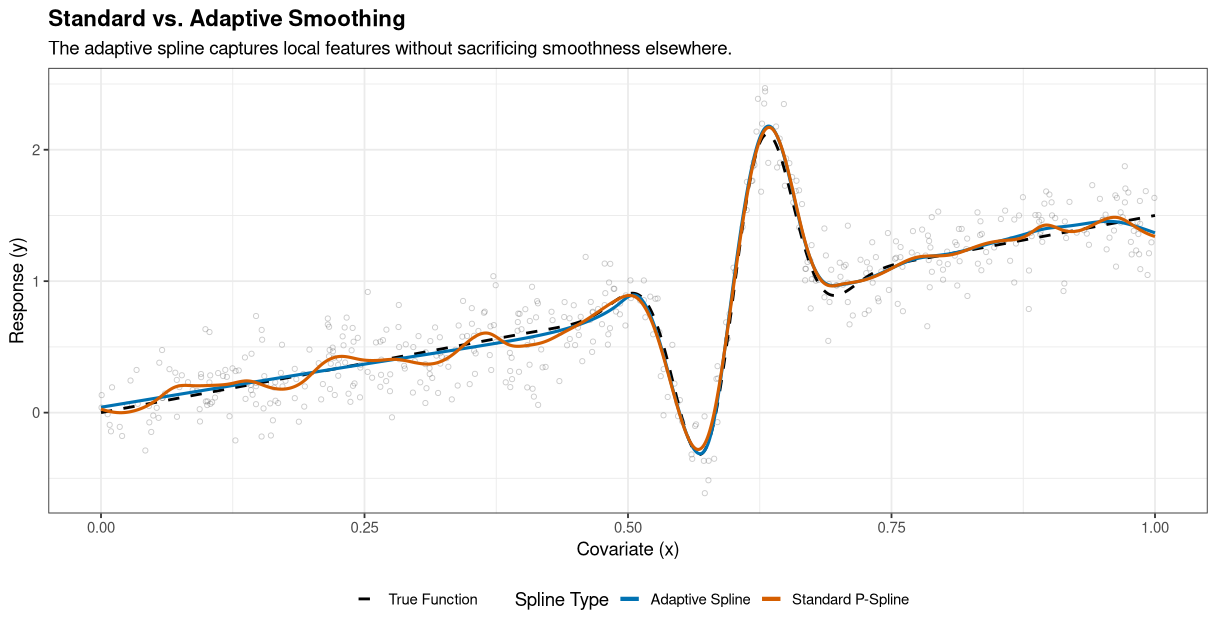
\includegraphics[width=\linewidth]{overviews//GAM-theory/adaptive_spline.png}
\end{figure}

\subsection{Spatially Varying Penalties and Adaptive Smoothing}

Standard smoothers assume constant smoothness across the entire domain, but real functions often exhibit varying complexity - smooth in some regions and rapidly changing in others. Adaptive smoothing addresses this by allowing the penalty strength to vary spatially.

\subsubsection{The Adaptive P-spline Framework}

\begin{definition}[Adaptive P-spline Penalty]
For a P-spline with basis coefficients $\boldsymbol{\beta} = (\beta_1, \ldots, \beta_K)^T$, the adaptive penalty is:
\begin{equation}
\mathcal{P}_a = \sum_{k=m}^{K} \omega_k (\Delta^m \beta_k)^2
\end{equation}
where:
\begin{itemize}
    \item $\Delta^m \beta_k$ is the $m$-th order difference of coefficients
    \item $\omega_k > 0$ are spatially-varying weights
    \item Each weight controls local penalty strength
\end{itemize}
\end{definition}

\subsubsection{Basis Expansion for Weights}

The crucial insight is to model the weights $\omega_k$ themselves using a basis expansion:

\begin{theorem}[Hierarchical Basis Structure]
Let the weights be represented as:
\begin{equation}
\boldsymbol{\omega} = \mathbf{B}\boldsymbol{\lambda}
\end{equation}
where:
\begin{itemize}
    \item $\mathbf{B}$ is an $K \times M$ basis matrix for the weights
    \item $\boldsymbol{\lambda} = (\lambda_1, \ldots, \lambda_M)^T$ are the basis coefficients
    \item $M \ll K$ typically (e.g., $M=5$ while $K=40$)
\end{itemize}
\end{theorem}

\begin{remark}[Positivity Constraint]
Since weights must be positive, we often work with:
\begin{equation}
\log(\omega_k) = \sum_{j=1}^M \gamma_j B_{kj} \quad \text{or} \quad \omega_k = \exp\left(\sum_{j=1}^M \gamma_j B_{kj}\right)
\end{equation}
\end{remark}

\subsubsection{Matrix Formulation and Multiple Smoothing Parameters}

\begin{theorem}[Decomposition into Multiple Penalties]
The adaptive penalty can be rewritten as a sum of $M$ separate penalties:
\begin{equation}
\mathcal{P}_a = \sum_{j=1}^M \lambda_j \boldsymbol{\beta}^T \mathbf{S}_j \boldsymbol{\beta}
\end{equation}
where each $\mathbf{S}_j$ is a penalty matrix.
\end{theorem}

\begin{proof}
Starting with the matrix form of the penalty:
\begin{align}
\mathcal{P}_a &= \boldsymbol{\beta}^T \mathbf{D}^T \text{diag}(\boldsymbol{\omega}) \mathbf{D} \boldsymbol{\beta}
\end{align}
where $\mathbf{D}$ is the $m$-th order difference matrix.

Substituting $\boldsymbol{\omega} = \mathbf{B}\boldsymbol{\lambda}$:
\begin{align}
\mathcal{P}_a &= \boldsymbol{\beta}^T \mathbf{D}^T \text{diag}(\mathbf{B}\boldsymbol{\lambda}) \mathbf{D} \boldsymbol{\beta} \\
&= \boldsymbol{\beta}^T \mathbf{D}^T \text{diag}\left(\sum_{j=1}^M \lambda_j \mathbf{B}_{.j}\right) \mathbf{D} \boldsymbol{\beta}
\end{align}
where $\mathbf{B}_{.j}$ denotes the $j$-th column of $\mathbf{B}$.

Using the linearity of the diagonal operator:
\begin{align}
\mathcal{P}_a &= \boldsymbol{\beta}^T \mathbf{D}^T \left(\sum_{j=1}^M \lambda_j \text{diag}(\mathbf{B}_{.j})\right) \mathbf{D} \boldsymbol{\beta} \\
&= \sum_{j=1}^M \lambda_j \boldsymbol{\beta}^T \mathbf{D}^T \text{diag}(\mathbf{B}_{.j}) \mathbf{D} \boldsymbol{\beta} \\
&= \sum_{j=1}^M \lambda_j \boldsymbol{\beta}^T \mathbf{S}_j \boldsymbol{\beta}
\end{align}
where $\mathbf{S}_j = \mathbf{D}^T \text{diag}(\mathbf{B}_{.j}) \mathbf{D}$.
\end{proof}

\subsubsection{Detailed Example: Second-Order Adaptive P-spline}

Consider a second-order penalty ($m=2$) with difference matrix:
\begin{equation}
\mathbf{D} = \begin{bmatrix}
1 & -2 & 1 & 0 & \cdots \\
0 & 1 & -2 & 1 & \cdots \\
\vdots & & \ddots & & \vdots
\end{bmatrix}
\end{equation}

For weight basis matrix $\mathbf{B}$ with $M=3$ basis functions:
\begin{equation}
\mathbf{B} = \begin{bmatrix}
B_{1,1} & B_{1,2} & B_{1,3} \\
B_{2,1} & B_{2,2} & B_{2,3} \\
\vdots & \vdots & \vdots \\
B_{K,1} & B_{K,2} & B_{K,3}
\end{bmatrix}
\end{equation}

The adaptive penalty becomes:
\begin{equation}
\mathcal{P}_a = \lambda_1 \boldsymbol{\beta}^T \mathbf{S}_1 \boldsymbol{\beta} + \lambda_2 \boldsymbol{\beta}^T \mathbf{S}_2 \boldsymbol{\beta} + \lambda_3 \boldsymbol{\beta}^T \mathbf{S}_3 \boldsymbol{\beta}
\end{equation}

Each $\mathbf{S}_j$ represents a different "aspect" of the penalty:
\begin{itemize}
    \item $\mathbf{S}_1$: Penalty weighted by first basis function of $\mathbf{B}$
    \item $\mathbf{S}_2$: Penalty weighted by second basis function
    \item $\mathbf{S}_3$: Penalty weighted by third basis function
\end{itemize}

\subsubsection{Implementation in mgcv}

\begin{definition}[mgcv Adaptive Smooth Specification]
In `mgcv`, an adaptive smooth is specified as:
\begin{verbatim}
s(x, bs="ad", k=40, m=5)
\end{verbatim}
where:
\begin{itemize}
    \item `k=40`: dimension of main smoothing basis (for $\boldsymbol{\beta}$)
    \item `m=5`: dimension of penalty basis (for weights)
    \item Results in 5 smoothing parameters $(\lambda_1, \ldots, \lambda_5)$
\end{itemize}
\end{definition}

\begin{algorithm}
\caption{Adaptive Smooth Construction in mgcv}
\begin{algorithmic}[1]
\State \textbf{Main Basis Construction:}
\State Create B-spline basis $\mathbf{X}$ of dimension $n \times k$ for main smooth
\State 
\State \textbf{Penalty Basis Construction:}
\State Create B-spline basis $\mathbf{B}$ of dimension $k \times m$ for penalty weights
\State Ensure $\mathbf{B}$ entries are non-negative (B-spline property)
\State 
\State \textbf{Multiple Penalty Matrices:}
\For{$j = 1$ to $m$}
    \State Extract $j$-th column: $\mathbf{b}_j = \mathbf{B}_{.j}$
    \State Form weight matrix: $\mathbf{W}_j = \text{diag}(\mathbf{b}_j)$
    \State Construct penalty: $\mathbf{S}_j = \mathbf{D}^T \mathbf{W}_j \mathbf{D}$
\EndFor
\State 
\State \textbf{Return:} Design matrix $\mathbf{X}$ and penalty matrices $\{\mathbf{S}_1, \ldots, \mathbf{S}_m\}$
\end{algorithmic}
\end{algorithm}

\subsubsection{Interpretation of Multiple Smoothing Parameters}

Each smoothing parameter $\lambda_j$ controls a different spatial pattern of smoothness:

\begin{example}[Univariate Adaptive Smooth]
Consider $s(x, \text{bs}=\text{"ad"}, k=30, m=4)$ with domain $x \in [0,1]$.

The penalty basis functions might be:
\begin{itemize}
    \item $B_1(x)$: Constant (uniform penalty)
    \item $B_2(x)$: Linear increasing (more penalty as $x$ increases)
    \item $B_3(x)$: Quadratic (penalty strong at ends, weak in middle)
    \item $B_4(x)$: Localized bump (penalty concentrated in specific region)
\end{itemize}

The estimated parameters might be:
\begin{itemize}
    \item $\hat{\lambda}_1 = 10$: Base level of smoothing
    \item $\hat{\lambda}_2 = 5$: Additional smoothing for large $x$
    \item $\hat{\lambda}_3 = -2$: Less smoothing in middle region
    \item $\hat{\lambda}_4 = 8$: Extra smoothing around bump location
\end{itemize}
\end{example}

\subsubsection{Effective Local Smoothing}

The effective local smoothing at position $x_i$ is:
\begin{equation}
\lambda_{\text{eff}}(x_i) = \sum_{j=1}^M \lambda_j B_j(x_i)
\end{equation}

This creates a smoothing parameter that varies continuously across the domain.

\subsubsection{Practical Considerations and Limitations}

\begin{remark}[Data Requirements]
Adaptive smoothing is data-hungry. With $M$ smoothing parameters, we effectively partition the data:
\begin{itemize}
    \item Each $\lambda_j$ is estimated from approximately $n/M$ effective observations
    \item For $n=200$ and $M=10$: like estimating 10 parameters from 20 observations each
    \item Recommendation: Use $M \leq 5$ unless $n$ is very large
\end{itemize}
\end{remark}

\begin{remark}[Identifiability Issues]
The model can become poorly identified if:
\begin{itemize}
    \item Penalty basis dimension $M$ is too large
    \item Main basis dimension $k$ is too small relative to $M$
    \item Data exhibits little variation in smoothness
\end{itemize}
\end{remark}

\subsubsection{Comparison with Standard P-splines}

\begin{table}[h]
\centering
\begin{tabular}{lll}
\toprule
\textbf{Aspect} & \textbf{Standard P-spline} & \textbf{Adaptive P-spline} \\
\midrule
Smoothing parameters & 1 & $M$ (e.g., 5) \\
Penalty structure & $\lambda \boldsymbol{\beta}^T \mathbf{S} \boldsymbol{\beta}$ & $\sum_{j=1}^M \lambda_j \boldsymbol{\beta}^T \mathbf{S}_j \boldsymbol{\beta}$ \\
Local flexibility & Constant & Spatially varying \\
Computational cost & $O(k^3)$ & $O(Mk^3)$ \\
Data requirements & Moderate & High \\
\bottomrule
\end{tabular}
\end{table}

\subsubsection{Alternative Parameterization}

In practice, `mgcv` often uses the parameterization:
\begin{equation}
\mathcal{P}_a = \boldsymbol{\beta}^T \left(\sum_{j=1}^M \lambda_j \mathbf{S}_j\right) \boldsymbol{\beta}
\end{equation}
where the combined penalty matrix is:
\begin{equation}
\mathbf{S}_{\text{total}} = \sum_{j=1}^M \lambda_j \mathbf{S}_j
\end{equation}

This allows the use of standard penalized regression machinery with multiple penalty matrices.

%% PART V: BAYESIAN CONNECTIONS %%
\part{Bayesian Connections and Inference}

\section{From Penalization to Priors}

\subsection{The Bayesian Model}

The connection between penalized estimation and Bayesian inference provides powerful tools for uncertainty quantification in GAMs.

\begin{theorem}[Penalized Splines as Bayesian Models]
The penalized least squares estimate is the posterior mode under:
\begin{align}
\mathbf{y} | \bm{\beta}, \sigma^2 &\sim N(\mathbf{X}\bm{\beta}, \sigma^2\mathbf{I}) \\
\bm{\beta} | \lambda, \sigma^2 &\sim N(\mathbf{0}, \sigma^2\lambda^{-1}\mathbf{S}^{-})
\end{align}
where $\mathbf{S}^{-}$ is a generalized inverse of $\mathbf{S}$.
\end{theorem}

\begin{proof}
The log-posterior is:
\begin{align}
\log p(\bm{\beta}|\mathbf{y}) &= \log p(\mathbf{y}|\bm{\beta}) + \log p(\bm{\beta}) + \text{const} \\
&= -\frac{1}{2\sigma^2}\|\mathbf{y} - \mathbf{X}\bm{\beta}\|^2 - \frac{\lambda}{2\sigma^2}\bm{\beta}^T\mathbf{S}\bm{\beta} + \text{const} \\
&= -\frac{1}{2\sigma^2}\left[\|\mathbf{y} - \mathbf{X}\bm{\beta}\|^2 + \lambda\bm{\beta}^T\mathbf{S}\bm{\beta}\right] + \text{const}
\end{align}

Maximizing the log-posterior is equivalent to minimizing the penalized least squares criterion.
\end{proof}

\textbf{GAM Insight:} This equivalence means:
\begin{itemize}
    \item The smoothing parameter $\lambda$ controls prior precision
    \item Larger $\lambda$ corresponds to stronger prior belief in smoothness
    \item The penalty matrix $\mathbf{S}$ defines the prior correlation structure
    \item Confidence bands have a Bayesian interpretation as credible intervals
\end{itemize}

\section{Posterior Distribution}

\subsection{Complete Posterior Derivation}

\begin{theorem}[Posterior Distribution of Coefficients]
Under the Bayesian model, the posterior distribution is:
\begin{equation}
\bm{\beta} | \mathbf{y}, \lambda, \sigma^2 \sim N(\hat{\bm{\beta}}, \mathbf{V}_\beta)
\end{equation}
where:
\begin{align}
\hat{\bm{\beta}} &= (\mathbf{X}^T\mathbf{X} + \lambda\mathbf{S})^{-1}\mathbf{X}^T\mathbf{y} \\
\mathbf{V}_\beta &= \sigma^2(\mathbf{X}^T\mathbf{X} + \lambda\mathbf{S})^{-1}
\end{align}
\end{theorem}

\begin{proof}
The log-posterior density is:
\begin{align}
\log p(\bm{\beta}|\mathbf{y}, \lambda, \sigma^2) &\propto -\frac{1}{2\sigma^2}\left[\|\mathbf{y} - \mathbf{X}\bm{\beta}\|^2 + \lambda\bm{\beta}^T\mathbf{S}\bm{\beta}\right]
\end{align}

Expanding the squared norm:
\begin{align}
&= -\frac{1}{2\sigma^2}\left[(\mathbf{y} - \mathbf{X}\bm{\beta})^T(\mathbf{y} - \mathbf{X}\bm{\beta}) + \lambda\bm{\beta}^T\mathbf{S}\bm{\beta}\right] \\
&= -\frac{1}{2\sigma^2}\left[\mathbf{y}^T\mathbf{y} - 2\mathbf{y}^T\mathbf{X}\bm{\beta} + \bm{\beta}^T\mathbf{X}^T\mathbf{X}\bm{\beta} + \lambda\bm{\beta}^T\mathbf{S}\bm{\beta}\right] \\
&= -\frac{1}{2\sigma^2}\left[\bm{\beta}^T(\mathbf{X}^T\mathbf{X} + \lambda\mathbf{S})\bm{\beta} - 2\mathbf{y}^T\mathbf{X}\bm{\beta} + \mathbf{y}^T\mathbf{y}\right]
\end{align}

To complete the square, we need to find $\hat{\bm{\beta}}$ such that:
\begin{equation}
\bm{\beta}^T(\mathbf{X}^T\mathbf{X} + \lambda\mathbf{S})\bm{\beta} - 2\mathbf{y}^T\mathbf{X}\bm{\beta} = (\bm{\beta} - \hat{\bm{\beta}})^T(\mathbf{X}^T\mathbf{X} + \lambda\mathbf{S})(\bm{\beta} - \hat{\bm{\beta}}) + \text{const}
\end{equation}

Expanding the right side:
\begin{align}
&(\bm{\beta} - \hat{\bm{\beta}})^T(\mathbf{X}^T\mathbf{X} + \lambda\mathbf{S})(\bm{\beta} - \hat{\bm{\beta}}) \\
&= \bm{\beta}^T(\mathbf{X}^T\mathbf{X} + \lambda\mathbf{S})\bm{\beta} - 2\bm{\beta}^T(\mathbf{X}^T\mathbf{X} + \lambda\mathbf{S})\hat{\bm{\beta}} + \hat{\bm{\beta}}^T(\mathbf{X}^T\mathbf{X} + \lambda\mathbf{S})\hat{\bm{\beta}}
\end{align}

Comparing coefficients of $\bm{\beta}$:
\begin{align}
-2\mathbf{y}^T\mathbf{X} &= -2\hat{\bm{\beta}}^T(\mathbf{X}^T\mathbf{X} + \lambda\mathbf{S}) \\
\mathbf{X}^T\mathbf{y} &= (\mathbf{X}^T\mathbf{X} + \lambda\mathbf{S})\hat{\bm{\beta}} \\
\hat{\bm{\beta}} &= (\mathbf{X}^T\mathbf{X} + \lambda\mathbf{S})^{-1}\mathbf{X}^T\mathbf{y}
\end{align}

Therefore:
\begin{equation}
\log p(\bm{\beta}|\mathbf{y}, \lambda, \sigma^2) \propto -\frac{1}{2\sigma^2}(\bm{\beta} - \hat{\bm{\beta}})^T(\mathbf{X}^T\mathbf{X} + \lambda\mathbf{S})(\bm{\beta} - \hat{\bm{\beta}})
\end{equation}

This is the log-density of $N(\hat{\bm{\beta}}, \sigma^2(\mathbf{X}^T\mathbf{X} + \lambda\mathbf{S})^{-1})$.
\end{proof}

\subsection{Handling the Null Space}

When $\mathbf{S}$ is rank-deficient (as is common), special care is needed for the null space components.

\begin{theorem}[Mixed Model Representation]
Decompose $\bm{\beta} = \mathbf{Z}\bm{\alpha} + \mathbf{W}\bm{\gamma}$ where:
\begin{itemize}
    \item $\mathbf{Z}$: basis for null space of $\mathbf{S}$ (unpenalized)
    \item $\mathbf{W}$: basis for range space of $\mathbf{S}$ (penalized)
\end{itemize}
Then:
\begin{align}
\bm{\alpha} &\sim \text{improper uniform prior} \\
\bm{\gamma} | \lambda, \sigma^2 &\sim N(\mathbf{0}, \sigma^2\lambda^{-1}\mathbf{I})
\end{align}
\end{theorem}

\textbf{GAM Interpretation:} The null space typically contains polynomial terms up to order $m-1$ (for an $m$-th derivative penalty). These terms are estimated without shrinkage, ensuring the smooth can represent polynomials exactly.

\section{Smoothing Parameter Selection}

\subsection{Generalized Cross-Validation (GCV)}

GCV provides a computationally efficient approximation to leave-one-out cross-validation.

\begin{definition}[GCV Score]
\begin{equation}
\mathcal{V}_g(\lambda) = \frac{n \cdot \text{RSS}(\lambda)}{[n - \tr(\mathbf{A}(\lambda))]^2}
\end{equation}
where $\text{RSS}(\lambda) = \|\mathbf{y} - \mathbf{A}(\lambda)\mathbf{y}\|^2$.
\end{definition}

\begin{theorem}[GCV Approximation to Leave-One-Out CV]
The leave-one-out CV score is:
\begin{equation}
\text{CV}(\lambda) = \frac{1}{n}\sum_{i=1}^n \left(\frac{y_i - \hat{y}_i(\lambda)}{1 - A_{ii}(\lambda)}\right)^2
\end{equation}
GCV approximates this by replacing $A_{ii}(\lambda)$ with $\bar{A} = \tr(\mathbf{A})/n$.
\end{theorem}

\textbf{Advantages for GAMs:}
\begin{itemize}
    \item Invariant to rotation in the response
    \item Computationally efficient (no need to refit $n$ times)
    \item Asymptotically optimal
    \item Works well for single smoothing parameters
\end{itemize}

\subsection{REML (Restricted Maximum Likelihood)}

\subsubsection{Mixed Model Representation of Penalized Splines}

To understand REML for smoothing parameter selection, we first establish the connection between penalized splines and linear mixed models.

\begin{theorem}[Penalized Splines as Mixed Models]
The penalized spline model:
\begin{equation}
\min_{\bm{\beta}} \left\{ \|\mathbf{y} - \mathbf{X}\bm{\beta}\|^2 + \lambda \bm{\beta}^T \mathbf{S} \bm{\beta} \right\}
\end{equation}
is equivalent to the linear mixed model:
\begin{align}
\mathbf{y} &= \mathbf{X}_f\bm{\beta}_f + \mathbf{X}_r\bm{\beta}_r + \bm{\epsilon} \\
\bm{\epsilon} &\sim N(\mathbf{0}, \sigma^2\mathbf{I}) \\
\bm{\beta}_r &\sim N(\mathbf{0}, \sigma^2_{\beta}\mathbf{I})
\end{align}
where the smoothing parameter is related to variance components by:
\begin{equation}
\lambda = \frac{\sigma^2}{\sigma^2_{\beta}}
\end{equation}
\end{theorem}

\begin{proof}
Decompose the coefficient vector using the eigen-decomposition of $\mathbf{S}$. Let $\mathbf{S} = \mathbf{U}\bm{\Lambda}\mathbf{U}^T$ where:
\begin{itemize}
    \item $\bm{\Lambda} = \text{diag}(0, \ldots, 0, \lambda_1, \ldots, \lambda_r)$ with $M$ zero eigenvalues
    \item $\mathbf{U} = [\mathbf{U}_0 | \mathbf{U}_r]$ where $\mathbf{U}_0$ spans the null space of $\mathbf{S}$
\end{itemize}

Reparameterize: $\bm{\beta} = \mathbf{U}_0\bm{\beta}_f + \mathbf{U}_r\bm{\beta}_r$ where:
\begin{itemize}
    \item $\bm{\beta}_f$: fixed effects (unpenalized)
    \item $\bm{\beta}_r$: random effects (penalized)
\end{itemize}

The penalty becomes:
\begin{equation}
\bm{\beta}^T\mathbf{S}\bm{\beta} = \bm{\beta}_r^T\bm{\Lambda}_r\bm{\beta}_r
\end{equation}

Setting $\mathbf{X}_f = \mathbf{X}\mathbf{U}_0$ and $\mathbf{X}_r = \mathbf{X}\mathbf{U}_r\bm{\Lambda}_r^{-1/2}$, and defining:
\begin{equation}
\tilde{\bm{\beta}}_r = \bm{\Lambda}_r^{1/2}\bm{\beta}_r \sim N(\mathbf{0}, \sigma^2\lambda^{-1}\mathbf{I})
\end{equation}

This gives the mixed model form with $\sigma^2_{\beta} = \sigma^2/\lambda$.
\end{proof}

\subsubsection{The Smoothing Parameter Trade-off}

The smoothing parameter $\lambda$ controls a fundamental trade-off:

\begin{definition}[Variance Component Interpretation]
The ratio $\lambda = \sigma^2/\sigma^2_{\beta}$ represents:
\begin{itemize}
    \item \textbf{Large $\lambda$ (small $\sigma^2_{\beta}$)}: Random effects have small variance
    \begin{itemize}
        \item Strong shrinkage toward zero
        \item Smooth functions (less flexibility)
        \item Bias-variance trade-off favors low variance
    \end{itemize}
    \item \textbf{Small $\lambda$ (large $\sigma^2_{\beta}$)}: Random effects have large variance
    \begin{itemize}
        \item Weak shrinkage
        \item Wiggly functions (more flexibility)
        \item Bias-variance trade-off favors low bias
    \end{itemize}
\end{itemize}
\end{definition}

\begin{remark}[Shrinkage Mechanism]
From the posterior mean $\hat{\bm{\beta}} = (\mathbf{X}^T\mathbf{X} + \lambda\mathbf{S})^{-1}\mathbf{X}^T\mathbf{y}$, we can see:
\begin{itemize}
    \item As $\lambda \to 0$: $\hat{\bm{\beta}} \to (\mathbf{X}^T\mathbf{X})^{-1}\mathbf{X}^T\mathbf{y}$ (unpenalized OLS)
    \item As $\lambda \to \infty$: $\hat{\bm{\beta}}$ is shrunk toward the null space of $\mathbf{S}$
\end{itemize}
\end{remark}

\subsubsection{The REML Criterion}

\begin{definition}[Marginal Likelihood]
The marginal likelihood integrates out the random effects:
\begin{equation}
L(\lambda, \sigma^2|\mathbf{y}) = \int p(\mathbf{y}|\bm{\beta}_f, \bm{\beta}_r, \sigma^2) p(\bm{\beta}_r|\sigma^2_{\beta}) d\bm{\beta}_r
\end{equation}
\end{definition}

For the mixed model representation:
\begin{equation}
\mathbf{y} \sim N(\mathbf{X}_f\bm{\beta}_f, \mathbf{V}_y)
\end{equation}
where the marginal covariance is:
\begin{equation}
\mathbf{V}_y = \sigma^2\mathbf{I} + \sigma^2_{\beta}\mathbf{X}_r\mathbf{X}_r^T = \sigma^2(\mathbf{I} + \lambda^{-1}\mathbf{X}_r\mathbf{X}_r^T)
\end{equation}

\begin{theorem}[REML Criterion Derivation]
The REML log-likelihood for $(\lambda, \sigma^2)$ is:
\begin{equation}
\ell_{REML}(\lambda, \sigma^2) = -\frac{1}{2}\left[\log|\mathbf{V}_y| + \log|\mathbf{X}_f^T\mathbf{V}_y^{-1}\mathbf{X}_f| + \mathbf{r}^T\mathbf{V}_y^{-1}\mathbf{r} + (n-p)\log(2\pi)\right]
\end{equation}
where:
\begin{itemize}
    \item $\mathbf{r} = \mathbf{y} - \mathbf{X}_f\hat{\bm{\beta}}_f$ are the residuals from fixed effects
    \item $\hat{\bm{\beta}}_f = (\mathbf{X}_f^T\mathbf{V}_y^{-1}\mathbf{X}_f)^{-1}\mathbf{X}_f^T\mathbf{V}_y^{-1}\mathbf{y}$
    \item $p = \text{rank}(\mathbf{X}_f)$ is the number of fixed effects
\end{itemize}
\end{theorem}

\begin{proof}
REML works with contrasts that remove fixed effects. Let $\mathbf{K}$ be an $(n-p) \times n$ matrix such that $\mathbf{K}\mathbf{X}_f = \mathbf{0}$ and $\mathbf{K}\mathbf{K}^T = \mathbf{I}_{n-p}$.

The contrasts $\mathbf{K}\mathbf{y} \sim N(\mathbf{0}, \mathbf{K}\mathbf{V}_y\mathbf{K}^T)$ have likelihood:
\begin{equation}
L_{REML} \propto |\mathbf{K}\mathbf{V}_y\mathbf{K}^T|^{-1/2} \exp\left(-\frac{1}{2}\mathbf{y}^T\mathbf{K}^T(\mathbf{K}\mathbf{V}_y\mathbf{K}^T)^{-1}\mathbf{K}\mathbf{y}\right)
\end{equation}

Using the identity $|\mathbf{K}\mathbf{V}_y\mathbf{K}^T| = |\mathbf{V}_y|/|\mathbf{X}_f^T\mathbf{V}_y^{-1}\mathbf{X}_f|$ and simplifying gives the result.
\end{proof}

\subsubsection{Why REML Over ML?}

\begin{theorem}[ML Bias in Variance Components]
Maximum likelihood estimation of $\sigma^2$ in the presence of fixed effects gives:
\begin{equation}
\hat{\sigma}^2_{ML} = \frac{1}{n}\sum_{i=1}^n (y_i - \hat{y}_i)^2
\end{equation}
which has expected value:
\begin{equation}
E[\hat{\sigma}^2_{ML}] = \frac{n-p}{n}\sigma^2 < \sigma^2
\end{equation}
REML corrects this bias by effectively using denominator $n-p$.
\end{theorem}

\subsubsection{Practical Implications of the Variance Component View}

\begin{enumerate}
\item \textbf{Multiple Smooth Terms}: For a model with multiple smooths:
\begin{equation}
f(x) = f_1(x_1) + f_2(x_2) + \cdots + f_k(x_k)
\end{equation}
Each smooth has its own variance component:
\begin{equation}
\lambda_j = \frac{\sigma^2}{\sigma^2_{\beta_j}}
\end{equation}
REML naturally handles this multivariate optimization.

\item \textbf{Smoothness Selection as Variance Partitioning}: REML answers: "How much variability in $\mathbf{y}$ should be attributed to:
\begin{itemize}
    \item Random noise ($\sigma^2$)?
    \item Smooth signal ($\sigma^2_{\beta}$)?
    \item Fixed effects (unpenalized)?"
\end{itemize}

\item \textbf{Connection to Effective Degrees of Freedom}:
\begin{equation}
\text{EDF} = \text{tr}(\mathbf{A}) \approx \frac{\text{Signal Variance}}{\text{Signal Variance} + \text{Noise Variance}/\lambda}
\end{equation}
As $\sigma^2_{\beta} \to 0$ (large $\lambda$), EDF approaches the dimension of the null space.
\end{enumerate}

\subsubsection{Computational Aspects}

\begin{algorithm}
\caption{REML Optimization for Smoothing Parameters}
\begin{algorithmic}[1]
\State Initialize $\lambda^{(0)}$, $\sigma^{2(0)}$
\Repeat
    \State Form $\mathbf{V}_y = \sigma^2(\mathbf{I} + \lambda^{-1}\mathbf{X}_r\mathbf{X}_r^T)$
    \State Compute Cholesky decomposition $\mathbf{V}_y = \mathbf{L}\mathbf{L}^T$
    \State Solve for $\hat{\bm{\beta}}_f$ using $\mathbf{L}$
    \State Evaluate REML gradient:
    \begin{equation}
    \frac{\partial \ell_{REML}}{\partial \lambda} = \frac{1}{2}\text{tr}\left[(\mathbf{P}\mathbf{X}_r\mathbf{X}_r^T)^2 - \mathbf{P}\mathbf{X}_r\mathbf{X}_r^T\right]\frac{1}{\lambda^2}
    \end{equation}
    where $\mathbf{P} = \mathbf{V}_y^{-1} - \mathbf{V}_y^{-1}\mathbf{X}_f(\mathbf{X}_f^T\mathbf{V}_y^{-1}\mathbf{X}_f)^{-1}\mathbf{X}_f^T\mathbf{V}_y^{-1}$
    \State Update $(\lambda, \sigma^2)$ using Newton-Raphson or Fisher scoring
\Until{convergence}
\end{algorithmic}
\end{algorithm}

\subsubsection{Summary: Why REML for GAMs}

\begin{itemize}
    \item Accounts for Uncertainty, as it does treat smooth terms as random effects with unknown variance
    \item Corrects the downward bias of ML for variance components
    \item Robustly handles models with many smooth terms
    \item Balances fit and smoothness through variance component estimation
    \item \textbf{Stability}: Generally more stable than GCV, especially for complex models
\end{itemize}



\subsection{Full Bayesian Approach}

For complete uncertainty quantification, we can place priors on the smoothing parameters themselves.

\begin{definition}[Hierarchical Bayesian Model]
\begin{align}
\text{Level 1:} \quad & \mathbf{y} | \bm{\beta}, \sigma^2 \sim N(\mathbf{X}\bm{\beta}, \sigma^2\mathbf{I}) \\
\text{Level 2:} \quad & \bm{\beta} | \lambda, \sigma^2 \sim N(\mathbf{0}, \sigma^2\lambda^{-1}\mathbf{S}^{-}) \\
\text{Level 3:} \quad & \lambda \sim \pi(\lambda), \quad \sigma^2 \sim \pi(\sigma^2)
\end{align}
\end{definition}

Common hyperprior choices:
\begin{itemize}
    \item $\lambda \sim \text{Gamma}(a_\lambda, b_\lambda)$ - conjugate, but can be informative
    \item $\sigma^2 \sim \text{Inverse-Gamma}(a_\sigma, b_\sigma)$ - standard conjugate prior
    \item $\tau = 1/\lambda \sim \text{Half-Cauchy}(0, \gamma)$ - robust, weakly informative
\end{itemize}

\textbf{GAM Benefits:}
\begin{itemize}
    \item Automatic complexity control
    \item Full posterior uncertainty including smoothing parameter uncertainty
    \item Coherent model comparison via marginal likelihoods
    \item Natural handling of hierarchical structures
\end{itemize}

\section{The Spline-Random Effect Duality}

This section reveals the deep connection between penalized splines and random effects, showing why mixed model software can fit GAMs.

\subsection{How Random Effects are Fitted as Splines (`bs="re"`)}

In mgcv, a random intercept term is just a special case of a penalized smooth.

\paragraph{The "Basis" and Penalty for a Random Effect}
For a factor `z` with $J$ levels:

\begin{enumerate}
    \item \textbf{The Model Matrix $\mathbf{X}$:} An $n \times J$ indicator matrix where $X_{ij} = 1$ if observation $i$ has level $j$
    
    \item \textbf{The Penalty Matrix $\mathbf{S}$:} Simply the $J \times J$ identity matrix, $\mathbf{S} = \mathbf{I}$
\end{enumerate}

The penalty term becomes:
\[ \lambda \boldsymbol{\beta}^T \mathbf{S} \boldsymbol{\beta} = \lambda \sum_{j=1}^{J} \beta_j^2 \]

This is exactly ridge regression on the group effects!

\paragraph{Connection to LMMs}
The smoothing parameter relates to variance components:
\[ \lambda = \frac{\sigma_e^2}{\sigma_b^2} \]
where $\sigma_e^2$ is the residual variance and $\sigma_b^2$ is the random effect variance.

\textbf{Key Insight:} Estimating $\lambda$ via REML is exactly equivalent to estimating variance components in a mixed model.

\subsection{Why All Penalized Splines are Random Effects}

We now show the general principle: any penalized spline can be viewed as a mixed model.

\subsubsection{Explicit Re-parameterization into Fixed and Random Components}

Starting with our penalized model:
\begin{equation*}
    \mathbf{y} = \mathbf{X}\boldsymbol{\beta} + \boldsymbol{\epsilon}, \quad \text{with penalty} \quad \lambda \boldsymbol{\beta}^T \mathbf{S} \boldsymbol{\beta}
\end{equation*}

Use the spectral decomposition of $\mathbf{S}$:
\begin{equation*}
    \mathbf{S} = \mathbf{U}\mathbf{D}\mathbf{U}^T
\end{equation*}

Split the eigenvectors:
\begin{itemize}
    \item $\mathbf{U}_f$: Eigenvectors for zero eigenvalues (null space)
    \item $\mathbf{U}_r$: Eigenvectors for positive eigenvalues (range space)
\end{itemize}

Re-parameterize:
\begin{equation*}
    \boldsymbol{\beta} = \mathbf{U}_f\boldsymbol{\alpha}_f + \mathbf{U}_r\boldsymbol{\alpha}_r
\end{equation*}

The model becomes:
\begin{equation*}
    \mathbf{y} = \underbrace{\mathbf{X}\mathbf{U}_f}_{\mathbf{X}_{fixed}}\boldsymbol{\alpha}_f + \underbrace{\mathbf{X}\mathbf{U}_r}_{\mathbf{Z}_{random}}\boldsymbol{\alpha}_r + \boldsymbol{\epsilon}
\end{equation*}

With the penalty only affecting the random part:
\begin{equation*}
    \lambda \boldsymbol{\beta}^T \mathbf{S} \boldsymbol{\beta} = \lambda \boldsymbol{\alpha}_r^T \mathbf{D}_r \boldsymbol{\alpha}_r
\end{equation*}

This is exactly a mixed model with:
\begin{itemize}
    \item Fixed effects: $\boldsymbol{\alpha}_f$ (unpenalized)
    \item Random effects: $\boldsymbol{\alpha}_r \sim N(\mathbf{0}, \sigma^2 \lambda^{-1} \mathbf{D}_r^{-1})$
\end{itemize}

\textbf{Profound Implication:} Every smooth term in a GAM can be reformulated as a combination of fixed effects (for the null space) and correlated random effects (for the penalized space). This justifies using mixed model methodology for all aspects of GAM fitting.

\newpage
\section{Case Study: Mathematical Formulation of a Binary GAMM}

We now apply all the theory to a concrete example: modeling malaria test results.

\subsection{Core Model Specification}

\subsubsection{1. Response Distribution}
Each individual's test result follows a Bernoulli distribution:
\begin{equation*}
    Y_i \mid p_i \sim \text{Bernoulli}(p_i)
\end{equation*}

\subsubsection{2. Link Function}
We use the logit link to ensure probabilities stay in [0,1]:
\begin{equation*}
    \text{logit}(p_i) = \log\left(\frac{p_i}{1-p_i}\right) = \eta_i
\end{equation*}

\subsubsection{3. Linear Predictor}
The linear predictor combines fixed effects, smooth terms, and random effects:
\begin{equation*}
    \eta_i = \beta_0 + \sum_{j=1}^{P} \beta_j x_{ij} + f(\text{age}_i) + b_{k(i)}
\end{equation*}

\textbf{Component Interpretation:}
\begin{itemize}
    \item $\beta_0$: Overall intercept (log-odds when all predictors = 0)
    \item $\beta_j x_{ij}$: Linear effects of covariates
    \item $f(\text{age}_i)$: Smooth nonlinear effect of age
    \item $b_{k(i)}$: Random intercept for village $k$
\end{itemize}

\subsection{Parameter Priors \& Distributional Assumptions}

\subsubsection{Fixed Effects ($\beta_j$)}
Flat priors (equivalent to maximum likelihood):
\begin{equation*}
    p(\beta_j) \propto 1
\end{equation*}

\subsubsection{Random Effect for Village ($b_k$)}
Villages are assumed exchangeable:
\begin{equation*}
    b_k \sim N(0, \sigma^2_v)
\end{equation*}

\textbf{Interpretation:} $\sigma^2_v$ measures between-village heterogeneity. Large $\sigma^2_v$ indicates substantial village-to-village variation in malaria risk.

\subsubsection{Smooth Function $f(\text{age})$: The Penalty as a Gaussian Prior}
The smooth is expanded in a B-spline basis:
\begin{equation*}
f(\text{age}) = \sum_{j=1}^{K} \gamma_j B_j(\text{age})
\end{equation*}

The penalty on the coefficients:
\begin{equation*}
    \text{Penalty} = \lambda \, \boldsymbol{\gamma}^T \mathbf{S} \boldsymbol{\gamma}
\end{equation*}

Is equivalent to the prior:
\begin{equation*}
    \boldsymbol{\gamma} \sim N(\mathbf{0}, (\lambda \mathbf{S})^{-})
\end{equation*}

\textbf{Key Insight:} The smoothing parameter $\lambda$ controls how strongly we believe the age effect should be smooth. REML estimates this from the data.

\subsection{Posterior Distribution and Inference}

After REML estimation of $\lambda$ and $\sigma_v^2$, we have:

\subsubsection{Posterior Distribution of Coefficients}
\begin{equation*}
    \boldsymbol{\theta} \mid \mathbf{y}, \lambda, \sigma_v^2 \sim N(\hat{\boldsymbol{\theta}}, \mathbf{V})
\end{equation*}

\subsubsection{Covariance Matrices in \texttt{mgcv}}
Three options with increasing conservatism:
\begin{enumerate}
    \item \textbf{The Frequentist Covariance Matrix ($\mathbf{V}_e$):} 
    \begin{itemize}
        \item Treats smoothing parameters as known constants
        \item Underestimates uncertainty
        \item Confidence intervals too narrow
    \end{itemize}

    \item \textbf{The Bayesian Posterior Covariance Matrix ($\mathbf{V}_p$):} 
    \begin{itemize}
        \item Default in `mgcv`
        \item Accounts for prior (penalty) but not uncertainty in $\lambda$
        \item Better than frequentist but still optimistic
    \end{itemize}

    \item \textbf{The "Unconditional" Covariance Matrix ($\mathbf{V}_c$):} 
    \begin{itemize}
        \item Corrects for smoothing parameter uncertainty
        \item Most accurate representation of total uncertainty
        \item Recommended for final inference
    \end{itemize}
\end{enumerate}

\begin{table}[h!]
\centering
\caption{Comparison of Covariance Matrices in GAMs (`mgcv`)}
\label{tab:covariance_matrices}
\begin{tabularx}{\linewidth}{>{\RaggedRight}p{1.5cm} >{\RaggedRight}p{2.2cm} >{\RaggedRight}p{2.5cm} >{\RaggedRight}X >{\RaggedRight\arraybackslash}X}
\toprule
\textbf{\texttt{mgcv} Object} & \textbf{Name} & \textbf{Statistical View} & \textbf{Key Feature} & \textbf{How to Access} \\
\midrule
\textbf{Ve} & Frequentist Covariance & Frequentist & Ignores smoothing parameter uncertainty. Can lead to over-confident (too narrow) intervals. & \texttt{vcov(gam\_model, freq = TRUE)} \\
\addlinespace
\textbf{Vp} & Bayesian Posterior Covariance & Bayesian (Conditional) & Default covariance. Bayesian posterior but is \textit{conditional} on the estimated smoothing parameters. & \texttt{vcov(gam\_model)} or \texttt{gam\_model\$Vp} \\
\addlinespace
\textbf{Vc} & Unconditional Covariance & Bayesian (Unconditional) & Corrected for smoothing parameter uncertainty. Provides more realistic, robust intervals. Generally preferred. However,  it breaks down (doesn't work as well) when the true function is close to the penalty null space of the smooth (see Marra and Wood 2012) & \texttt{vcov(gam\_model, unconditional = TRUE)} \\
\bottomrule
\end{tabularx}
\end{table}


\subsubsection{Derivation of the Corrected (Unconditional) Covariance Matrix}

The key insight is that the standard Bayesian posterior covariance ignores the fact that smoothing parameters $\lambda$ were estimated from the data, not known a priori.

\paragraph{The Problem with Conditional Covariance}
The standard Bayesian posterior covariance is:
\begin{equation}
\mathbf{V}_p = \hat{\sigma}^2(\mathbf{X}^T\mathbf{X} + \hat{\lambda}\mathbf{S})^{-1}
\end{equation}
This treats $\hat{\lambda}$ as fixed, but in reality $\lambda$ has uncertainty from estimation.

\paragraph{Correcting for Smoothing Parameter Uncertainty}
Following Wood (2016) and the methods in the document, the corrected covariance incorporates uncertainty in $\lambda$ through a first-order Taylor expansion:

\begin{equation}
\mathbf{V}_c = \mathbf{V}_p + \mathbf{V}_\lambda + \mathbf{V}_{\lambda\lambda}
\end{equation}

where:
\begin{itemize}
    \item $\mathbf{V}_p$ is the standard posterior covariance (conditional on $\hat{\lambda}$)
    \item $\mathbf{V}_\lambda$ accounts for first-order uncertainty in $\lambda$
    \item $\mathbf{V}_{\lambda\lambda}$ accounts for second-order effects
\end{itemize}

\paragraph{Detailed Components}

\textbf{1. First-order correction:}
\begin{equation}
\mathbf{V}_\lambda = \mathbf{J}\mathbf{V}_\rho\mathbf{J}^T
\end{equation}
where:
\begin{itemize}
    \item $\mathbf{J} = \frac{\partial\hat{\boldsymbol{\beta}}}{\partial\boldsymbol{\rho}}\bigg|_{\hat{\boldsymbol{\rho}}}$ is the Jacobian matrix showing how coefficient estimates change with log smoothing parameters
    \item $\mathbf{V}_\rho$ is the covariance matrix of $\boldsymbol{\rho} = \log(\boldsymbol{\lambda})$ from REML
\end{itemize}

\textbf{2. Second-order correction:}
\begin{equation}
(\mathbf{V}_{\lambda\lambda})_{jm} = \sum_{p} \sum_{i} \sum_{l} \sum_{k} \frac{\partial R_{ij}}{\partial\rho_k} V_{\rho,kl} \frac{\partial R_{im}}{\partial\rho_l}
\end{equation}
where $\mathbf{R}$ comes from the Cholesky decomposition $\mathbf{V}_p = \mathbf{R}^T\mathbf{R}$.

\paragraph{Computing the Jacobian}
The key computational challenge is obtaining $\mathbf{J}$. Using implicit differentiation at the penalized likelihood maximum:
\begin{equation}
\frac{\partial\hat{\beta}_i}{\partial\rho_k} = (\mathbf{X}^T\mathbf{X} + \lambda\mathbf{S})^{-1}_{ij} \lambda_k S^k_{jl} \hat{\beta}_l
\end{equation}

\paragraph{The Complete Corrected Covariance}
The full unconditional covariance matrix becomes:
\begin{equation}
\boxed{\mathbf{V}_c = \mathbf{V}_p + \mathbf{J}\mathbf{V}_\rho\mathbf{J}^T + \mathbf{V}_{\lambda\lambda}}
\end{equation}

\paragraph{Practical Impact}
\begin{itemize}
    \item The correction typically increases the variance (wider confidence bands)
    \item The effect is larger when:
        \begin{itemize}
            \item Sample size is small
            \item Smoothing parameters are poorly identified
            \item The smooth is near the boundary (very smooth or very wiggly)
        \end{itemize}
\end{itemize}

\paragraph{Implementation in mgcv}
The \texttt{mgcv} package computes this automatically when you specify:
\begin{verbatim}
vcov(model, unconditional = TRUE)
\end{verbatim}

This correction ensures that confidence intervals have proper coverage when smoothing parameters are estimated from the data, not known a priori.

\subsubsection{Simulating the Smooth Effect}
To visualize uncertainty in $f(\text{age})$:

\begin{enumerate}
    \item \textbf{Obtain Estimates:} Extract $\hat{\boldsymbol{\theta}}$ and $\mathbf{V}_c$
    
    \item \textbf{Generate Prediction Grid:} Create dense age values
    
    \item \textbf{Draw from the Posterior:} 
    \begin{equation*}
        \boldsymbol{\theta}^{(m)} \sim N(\hat{\boldsymbol{\theta}}, \mathbf{V}_c) \quad \text{for } m = 1, \dots, M
    \end{equation*}
    
    \item \textbf{Predict Smooth Realizations:} 
    \begin{equation*}
        \mathbf{f}^{(m)} = \mathbf{X}_p \boldsymbol{\theta}^{(m)}
    \end{equation*}
    
    \item \textbf{Calculate Confidence Bands:} Use 2.5\% and 97.5\% quantiles
\end{enumerate}





\subsection{Pointwise vs. Simultaneous Confidence Intervals}

\subsubsection{Fundamental Distinction}

When constructing confidence intervals for smooth functions in GAMs, we must distinguish between two fundamentally different types of coverage:

\begin{definition}[Pointwise Confidence Intervals]
For a smooth function $f: \mathcal{X} \to \mathbb{R}$ at confidence level $1-\alpha$, pointwise confidence intervals satisfy:
\begin{equation}
P\left(f(x) \in [L_p(x), U_p(x)]\right) = 1-\alpha \quad \text{for each fixed } x \in \mathcal{X}
\end{equation}
where $L_p(x)$ and $U_p(x)$ are the lower and upper pointwise bounds at $x$.
\end{definition}

\begin{definition}[Simultaneous Confidence Bands]
Simultaneous confidence bands at level $1-\alpha$ satisfy:
\begin{equation}
P\left(f(x) \in [L_s(x), U_s(x)] \text{ for all } x \in \mathcal{X}\right) = 1-\alpha
\end{equation}
where the probability statement holds for the entire function over the domain $\mathcal{X}$.
\end{definition}

\begin{remark}[Critical Distinction]
The key difference is:
\begin{itemize}
   \item Pointwise: $\forall x \in \mathcal{X}: P(f(x) \in \text{CI}(x)) = 1-\alpha$ (separate statements)
   \item Simultaneous: $P(\forall x \in \mathcal{X}: f(x) \in \text{CB}(x)) = 1-\alpha$ (joint statement)
\end{itemize}
\end{remark}

\subsubsection{Construction from Posterior Samples}

Given posterior samples $\{f^{(b)}(x)\}_{b=1}^B$ where $f^{(b)}(x) = \sum_k \beta_k^{(b)} B_k(x)$:

\begin{theorem}[Pointwise Interval Construction]
The $(1-\alpha)$ pointwise credible interval at $x$ is:
\begin{equation}
[L_p(x), U_p(x)] = \left[Q_{\alpha/2}\{f^{(b)}(x)\}, Q_{1-\alpha/2}\{f^{(b)}(x)\}\right]
\end{equation}
where $Q_p\{\cdot\}$ denotes the $p$-th empirical quantile over samples $b = 1, \ldots, B$.
\end{theorem}

\begin{theorem}[Simultaneous Band Construction via Supremum]
Define the standardized deviation:
\begin{equation}
Z^{(b)}(x) = \frac{f^{(b)}(x) - \hat{f}(x)}{\text{se}(f(x))}
\end{equation}
where $\hat{f}(x) = \mathbb{E}[f(x)|\mathbf{y}]$ and $\text{se}(f(x)) = \sqrt{\text{Var}(f(x)|\mathbf{y})}$.

The simultaneous bands are:
\begin{equation}
[L_s(x), U_s(x)] = \hat{f}(x) \pm q_{1-\alpha} \cdot \text{se}(f(x))
\end{equation}
where $q_{1-\alpha}$ is the $(1-\alpha)$-quantile of $\sup_{x \in \mathcal{X}} |Z^{(b)}(x)|$.
\end{theorem}

\subsubsection{Theoretical Properties}

\begin{proposition}[Coverage Probability Relationship]
For any smooth function $f$ and domain $\mathcal{X}$ with more than one point:
\begin{equation}
P(\text{simultaneous coverage}) < P(\text{pointwise coverage at all observed points})
\end{equation}
with equality only in degenerate cases.
\end{proposition}

\begin{proof}
Let $A_x = \{f(x) \in [L_p(x), U_p(x)]\}$ be the event of coverage at $x$. Then:
\begin{align}
P\left(\bigcap_{x \in \mathcal{X}} A_x\right) &\leq P(A_x) = 1-\alpha \quad \text{for any } x \\
P\left(\bigcap_{x \in \mathcal{X}} A_x\right) &< 1-\alpha \quad \text{when } A_x \text{ are not perfectly correlated}
\end{align}
\end{proof}

\begin{theorem}[Asymptotic Width Ratio ]
Under regularity conditions, as the sample size $n \to \infty$:
\begin{equation}
\frac{\text{Width}_{\text{simultaneous}}(x)}{\text{Width}_{\text{pointwise}}(x)} \approx \frac{q_{1-\alpha}}{z_{1-\alpha/2}}
\end{equation}
where:
\begin{itemize}
   \item $z_{1-\alpha/2} = \Phi^{-1}(1-\alpha/2)$ is the standard normal quantile (e.g., 1.96 for $\alpha=0.05$)
   \item $q_{1-\alpha}$ is the $(1-\alpha)$-quantile of $\sup_{x \in \mathcal{X}} |W(x)|$
   \item $W(x)$ is a mean-zero Gaussian process with covariance structure inherited from the smoother
\end{itemize}
\end{theorem}

\begin{remark}[More on $q_{1-\alpha}$]
The quantity $q_{1-\alpha}$ arises from the distribution of the maximum absolute value of a Gaussian process:

\textbf{Step 1: Standardized Process}
Under the null hypothesis and asymptotic normality:
\begin{equation}
\frac{f(x) - \mathbb{E}[f(x)|\mathbf{y}]}{\sqrt{\text{Var}(f(x)|\mathbf{y})}} \approx W(x)
\end{equation}
where $W(x)$ is a Gaussian process with correlation structure determined by the smoother.

\textbf{Step 2: Supremum Distribution}
To achieve simultaneous coverage, we need:
\begin{equation}
P\left(\sup_{x \in \mathcal{X}} |W(x)| \leq q_{1-\alpha}\right) = 1-\alpha
\end{equation}

\textbf{Step 3: Dependence on Smoother Complexity}
The value of $q_{1-\alpha}$ depends on:
\begin{itemize}
   \item \textbf{Effective degrees of freedom (EDF)}: Higher EDF $\Rightarrow$ larger $q_{1-\alpha}$
   \item \textbf{Correlation structure}: Smoother functions $\Rightarrow$ smaller $q_{1-\alpha}$
   \item \textbf{Domain size}: Larger domain $\Rightarrow$ larger $q_{1-\alpha}$
\end{itemize}
\end{remark}

\begin{example}[Concrete Values of $q_{1-\alpha}$]
For $\alpha = 0.05$ (95\% confidence):
\begin{itemize}
   \item \textbf{Simple case}: Linear regression (EDF = 2)
   \begin{equation}
   q_{0.95} \approx \sqrt{\chi^2_{2,0.95}} \approx 2.45
   \end{equation}
   
   \item \textbf{Smooth with EDF = 4}:
   \begin{equation}
   q_{0.95} \approx 2.6 \text{ to } 2.8
   \end{equation}
   
   \item \textbf{Complex smooth with EDF = 10}:
   \begin{equation}
   q_{0.95} \approx 3.0 \text{ to } 3.3
   \end{equation}
\end{itemize}
Compare to $z_{0.975} = 1.96$ for pointwise intervals.
\end{example}

\begin{theorem}[Exact Form of $q_{1-\alpha}$ for Special Cases]
\textbf{Case 1: Polynomial Regression}
For a polynomial of degree $d$ (EDF = $d+1$):
\begin{equation}
q_{1-\alpha} = \sqrt{F_{d+1,n-d-1,1-\alpha} \cdot (d+1)}
\end{equation}
where $F_{d+1,n-d-1,1-\alpha}$ is the F-distribution quantile.

\textbf{Case 2: Penalized Spline (Approximate)}
For a penalized spline with EDF = $\nu$:
\begin{equation}
q_{1-\alpha} \approx \sqrt{2\log\left(\frac{\nu}{\sqrt{2\pi}}\right) + \chi^2_{1,1-\alpha}}
\end{equation}
This approximation uses extreme value theory for Gaussian processes.
\end{theorem}

\begin{remark}[Practical Interpretation]
The ratio $\frac{q_{1-\alpha}}{z_{1-\alpha/2}}$ tells us:
\begin{itemize}
   \item \textbf{For EDF $\approx$ 4}: Simultaneous bands are $\approx$ 40\% wider than pointwise
   \item \textbf{For EDF $\approx$ 10}: Simultaneous bands are $\approx$ 60\% wider than pointwise
   \item \textbf{General rule}: Width multiplier $\approx 1.3$ to $1.7$ for typical smooths
\end{itemize}

This extra width is the "price" of making statements about the entire function rather than individual points.
\end{remark}

\begin{algorithm}
\caption{Estimating $q_{1-\alpha}$ via Simulation}
\begin{algorithmic}[1]
\State \textbf{Input:} Fitted GAM, confidence level $1-\alpha$
\State Extract: $\hat{\boldsymbol{\beta}}$, $\mathbf{V}_\beta = \text{Cov}(\boldsymbol{\beta}|\mathbf{y})$
\State Define fine grid: $\{x_1, \ldots, x_G\}$ over domain
\For{$s = 1$ to $S$ (e.g., $S = 10000$)}
   \State Draw $\boldsymbol{\beta}^{(s)} \sim N(\hat{\boldsymbol{\beta}}, \mathbf{V}_\beta)$
   \State Compute $f^{(s)}(x_i) = \mathbf{B}(x_i)^T\boldsymbol{\beta}^{(s)}$ for all $i$
   \State Compute $Z^{(s)}(x_i) = \frac{f^{(s)}(x_i) - \hat{f}(x_i)}{\text{se}(f(x_i))}$
   \State $M^{(s)} = \max_{i=1,\ldots,G} |Z^{(s)}(x_i)|$
\EndFor
\State $\hat{q}_{1-\alpha} = \text{quantile}_{1-\alpha}\{M^{(1)}, \ldots, M^{(S)}\}$
\State \textbf{Return:} $\hat{q}_{1-\alpha}$
\end{algorithmic}
\end{algorithm}

\begin{example}[Why $q_{1-\alpha} > z_{1-\alpha/2}$]
Consider testing if $f(x) = 0$ at 100 equally spaced points:
\begin{itemize}
   \item \textbf{Pointwise}: Each test uses critical value $z_{0.975} = 1.96$
   \item \textbf{Expected false positives}: $100 \times 0.05 = 5$ points
   \item \textbf{Simultaneous}: Need $P(\text{no false positives}) = 0.95$
   \item \textbf{Required}: Larger critical value $q_{0.95} \approx 2.8$
\end{itemize}
The increase from 1.96 to 2.8 ensures we control the family-wise error rate.
\end{example}

\subsubsection{Practical Multipliers for Simultaneous Bands}

\begin{definition}[Simultaneous Coverage Multiplier]
The multiplier $c_\alpha$ that converts pointwise to simultaneous bands:
\begin{equation}
\text{Simultaneous CI} = \hat{f}(x) \pm c_\alpha \cdot \text{se}(f(x))
\end{equation}
where $c_\alpha > z_{1-\alpha/2}$.
\end{definition}

\begin{proposition}[Multiplier Bounds]
For a smooth with effective degrees of freedom $\nu$:
\begin{equation}
z_{1-\alpha/2} < c_\alpha < \sqrt{\chi^2_{\nu,1-\alpha}}
\end{equation}
with the upper bound being conservative.
\end{proposition}

\subsubsection{Multiple Testing Interpretation}

\begin{theorem}[Bonferroni Lower Bound]
If evaluating the function at $m$ points, the Bonferroni correction gives:
\begin{equation}
P\left(\bigcap_{i=1}^m \{f(x_i) \in \text{CI}_{\alpha/m}(x_i)\}\right) \geq 1-\alpha
\end{equation}
This provides conservative simultaneous coverage over the finite set $\{x_1, \ldots, x_m\}$.
\end{theorem}

\subsubsection{When to Use Each Type}

\begin{table}[h]
\centering
\begin{tabular}{lll}
\toprule
\textbf{Scenario} & \textbf{Appropriate Type} & \textbf{Rationale} \\
\midrule
Testing $f(x_0) = 0$ at specific $x_0$ & Pointwise & Single hypothesis \\
Testing if $f$ is flat everywhere & Simultaneous & Multiple hypotheses \\
Identifying regions where $f(x) > 0$ & Simultaneous & Avoids false discoveries \\
Predicting at new $x_{\text{new}}$ & Pointwise & Single prediction \\
Publishing function estimate & Simultaneous & Scientific rigor \\
Clinical decision at age 50 & Pointwise & Specific point \\
\bottomrule
\end{tabular}
\end{table}

\subsubsection{Implementation in GAMs}

\begin{algorithm}
\caption{Computing Both Types of Confidence Intervals}
\begin{algorithmic}[1]
\State \textbf{Input:} Posterior samples $\{\boldsymbol{\beta}^{(b)}\}_{b=1}^B$, evaluation points $\{x_i\}_{i=1}^n$
\State \textbf{Step 1: Compute function samples}
\For{$b = 1$ to $B$}
   \For{$i = 1$ to $n$}
       \State $f^{(b)}(x_i) = \sum_k \beta_k^{(b)} B_k(x_i)$
   \EndFor
\EndFor
\State 
\State \textbf{Step 2: Pointwise intervals}
\For{$i = 1$ to $n$}
   \State $L_p(x_i) = \text{quantile}_{\alpha/2}\{f^{(1)}(x_i), \ldots, f^{(B)}(x_i)\}$
   \State $U_p(x_i) = \text{quantile}_{1-\alpha/2}\{f^{(1)}(x_i), \ldots, f^{(B)}(x_i)\}$
\EndFor
\State 
\State \textbf{Step 3: Simultaneous bands}
\State Compute $\hat{f}(x_i) = \frac{1}{B}\sum_b f^{(b)}(x_i)$ and $\text{se}(x_i)$
\For{$b = 1$ to $B$}
   \State $M^{(b)} = \max_i |f^{(b)}(x_i) - \hat{f}(x_i)|/\text{se}(x_i)$
\EndFor
\State $c_\alpha = \text{quantile}_{1-\alpha}\{M^{(1)}, \ldots, M^{(B)}\}$
\For{$i = 1$ to $n$}
   \State $L_s(x_i) = \hat{f}(x_i) - c_\alpha \cdot \text{se}(x_i)$
   \State $U_s(x_i) = \hat{f}(x_i) + c_\alpha \cdot \text{se}(x_i)$
\EndFor
\end{algorithmic}
\end{algorithm}

\begin{remark}[Software Implementation]
In \texttt{mgcv}:
\begin{itemize}
   \item \texttt{plot.gam(...)} produces pointwise intervals (default)
   \item \texttt{plot.gam(..., seWithMean=TRUE)} includes uncertainty in the mean
   \item Custom code needed for exact simultaneous bands
   \item Approximate simultaneous bands: multiply standard errors by $\sqrt{\text{EDF}}$
\end{itemize}
\end{remark}

\subsubsection{Common Misinterpretations}

\begin{example}[Incorrect Interpretation of Pointwise Bands]
\textbf{Wrong:} "We are 95\% confident the true function lies entirely within these bands."

\textbf{Correct:} "At any single point we choose to examine, we are 95\% confident the true function value lies within the bands at that point."
\end{example}

\begin{example}[False Discovery with Pointwise Bands]
When examining where $f(x) \neq 0$ using pointwise 95\% intervals:
\begin{itemize}
   \item Expected false discoveries: $\approx 5\%$ of examined points
   \item With 100 points tested: $\approx 5$ false rejections expected
   \item Simultaneous bands control family-wise error rate
\end{itemize}
\end{example}

\begin{remark}[Conservative Nature of Simultaneous Bands]
Simultaneous bands are often conservative because:
\begin{enumerate}
   \item They must cover the entire function, including unobserved points
   \item The supremum distribution has heavier tails than pointwise distributions
   \item Correlation between nearby points is not fully exploited
\end{enumerate}
This conservatism is the price of making global statements about the function.
\end{remark}

\section{Algorithms for Posterior Sampling and Derivatives}

\subsection{Posterior Sampling from Penalized Splines}

\subsubsection{The Hierarchical Model Structure}

Penalized splines naturally arise from a three-level hierarchical model:
\begin{align}
\text{Level 1 (Data):} \quad & \mathbf{y} | \boldsymbol{\beta}, \sigma^2 \sim N(\mathbf{X}\boldsymbol{\beta}, \sigma^2\mathbf{I}) \\
\text{Level 2 (Coefficients):} \quad & \boldsymbol{\beta} | \lambda, \sigma^2 \sim N(\mathbf{0}, \sigma^2\lambda^{-1}\mathbf{S}^{-}) \\
\text{Level 3 (Hyperparameters):} \quad & \lambda, \sigma^2 \sim \pi(\lambda, \sigma^2)
\end{align}

The treatment of hyperparameters $\lambda$ and $\sigma^2$ distinguishes different inferential approaches.

\subsubsection{Empirical Bayes Approach (Standard in Practice)}

Empirical Bayes estimates hyperparameters by maximizing the marginal likelihood after integrating out $\boldsymbol{\beta}$.

\begin{definition}[Empirical Bayes Framework]
The approach proceeds in three steps:
\begin{enumerate}
    \item \textbf{Marginalization:} Integrate out coefficients to obtain
    \begin{equation}
    p(\mathbf{y}|\lambda, \sigma^2) = \int p(\mathbf{y}|\boldsymbol{\beta}, \sigma^2) p(\boldsymbol{\beta}|\lambda, \sigma^2) d\boldsymbol{\beta}
    \end{equation}
    
    \item \textbf{Optimization:} Find hyperparameter estimates
    \begin{equation}
    (\hat{\lambda}, \hat{\sigma}^2) = \argmax_{(\lambda, \sigma^2)} p(\mathbf{y}|\lambda, \sigma^2)
    \end{equation}
    typically using REML to reduce bias in variance components.
    
    \item \textbf{Plug-in Posterior:} Condition on estimates to obtain
    \begin{equation}
    \boldsymbol{\beta} | \mathbf{y}, \hat{\lambda}, \hat{\sigma}^2 \sim N(\hat{\boldsymbol{\beta}}, \mathbf{V}_{\beta})
    \end{equation}
    where:
    \begin{align}
    \hat{\boldsymbol{\beta}} &= (\mathbf{X}^T\mathbf{X} + \hat{\lambda}\mathbf{S})^{-1}\mathbf{X}^T\mathbf{y} \\
    \mathbf{V}_{\beta} &= \hat{\sigma}^2(\mathbf{X}^T\mathbf{X} + \hat{\lambda}\mathbf{S})^{-1}
    \end{align}
\end{enumerate}
\end{definition}

\begin{remark}[Advantages of Empirical Bayes]
\begin{itemize}
    \item Computationally efficient (seconds vs. hours)
    \item Leverages established mixed model theory
    \item Implemented in standard software (`mgcv`)
    \item Limitation: Underestimates uncertainty by treating $\hat{\lambda}$ as fixed
\end{itemize}
\end{remark}

\subsubsection{Fully Bayesian Approach (Complete Inference)}

The fully Bayesian approach specifies priors on hyperparameters and samples from the complete posterior.

\begin{definition}[Fully Bayesian Framework]
Specify hyperprior distributions:
\begin{align}
\lambda &\sim \text{Gamma}(a_\lambda, b_\lambda) \quad \text{or} \quad \tau = 1/\lambda \sim \text{Half-Cauchy}(0, \gamma) \\
\sigma^2 &\sim \text{Inverse-Gamma}(a_\sigma, b_\sigma)
\end{align}

Target the joint posterior:
\begin{equation}
p(\boldsymbol{\beta}, \lambda, \sigma^2 | \mathbf{y}) \propto p(\mathbf{y}|\boldsymbol{\beta}, \sigma^2) p(\boldsymbol{\beta}|\lambda, \sigma^2) p(\lambda) p(\sigma^2)
\end{equation}

Sample via MCMC (implemented in `brms`, `rstanarm`, `INLA`).
\end{definition}

\begin{remark}[When to Use Fully Bayesian]
Essential when:
\begin{itemize}
    \item Hyperparameter uncertainty substantially affects conclusions
    \item Sample size is small (asymptotic approximations fail)
    \item Prior information should be incorporated
    \item Complete uncertainty quantification is critical
\end{itemize}
\end{remark}

\subsection{Practical Algorithms for Posterior Sampling}

\subsubsection{Algorithm 1: Gaussian Approximation (Standard Approach)}

This algorithm implements Empirical Bayes with optional correction for smoothing parameter uncertainty.

\begin{algorithm}[H]
\caption{Posterior Sampling via Gaussian Approximation}
\begin{algorithmic}[1]
\State \textbf{Input:} Fitted GAM model, number of samples $B$
\State Extract estimates: $\hat{\boldsymbol{\beta}} = \text{coef(model)}$, $\hat{\lambda}$ from model fit
\State Estimate residual variance: $\hat{\sigma}^2 = \frac{\text{RSS}}{n - \text{tr}(\mathbf{A})}$
\State \textbf{Choose covariance matrix:}
\State \quad Option 1 (Conditional): $\mathbf{V} = \hat{\sigma}^2(\mathbf{X}^T\mathbf{X} + \hat{\lambda}\mathbf{S})^{-1}$
\State \quad Option 2 (Corrected): $\mathbf{V} = \text{vcov(model, unconditional = TRUE)}$
\State \quad \quad \textit{(partially accounts for uncertainty in $\hat{\lambda}$)}
\For{$b = 1$ to $B$}
    \State Draw $\boldsymbol{\beta}^{(b)} \sim N(\hat{\boldsymbol{\beta}}, \mathbf{V})$
    \State Compute predictions: $\hat{\mathbf{y}}^{(b)} = \mathbf{X}\boldsymbol{\beta}^{(b)}$
\EndFor
\State \textbf{Return:} Posterior samples $\{\boldsymbol{\beta}^{(b)}\}_{b=1}^B$
\end{algorithmic}
\end{algorithm}

\begin{remark}[Frequentist Interpretation]
When viewed frequentistically:
\begin{itemize}
    \item $\hat{\lambda}$ is a fixed constant (not random)
    \item Use only conditional covariance (Option 1)
    \item Samples represent uncertainty in $\boldsymbol{\beta}$ given fixed smoothing
    \item Confidence intervals are narrower than Bayesian credible intervals
\end{itemize}
\end{remark}

\subsubsection{Algorithm 2: Metropolis-Hastings with Mixed Proposals}

When the Gaussian approximation is inadequate, `gam.mh` uses a sophisticated hybrid sampler.

\begin{algorithm}[H]
\caption{Metropolis-Hastings for GAMs (Wood, 2015)}
\begin{algorithmic}[1]
\State \textbf{Input:} GAM model, samples `ns`, burn-in `burn`, `t.df`, `rw.scale`
\State Extract: $\hat{\boldsymbol{\beta}} = \text{coef(model)}$, $\mathbf{V} = \text{vcov(model)}$
\State Initialize: $\boldsymbol{\beta}_{\text{current}} = \hat{\boldsymbol{\beta}}$
\For{$i = 1$ to `burn` + `ns`}
    \State \textbf{Step 1: Fixed Proposal}
    \State \quad Draw $\boldsymbol{\beta}_{\text{prop}} \sim t_{\text{t.df}}(\hat{\boldsymbol{\beta}}, \mathbf{V})$
    \State \quad Compute acceptance probability:
    \begin{equation}
    \alpha_{\text{fixed}} = \min\left(1, \frac{p(\boldsymbol{\beta}_{\text{prop}}|\mathbf{y}) \cdot t(\boldsymbol{\beta}_{\text{current}}; \hat{\boldsymbol{\beta}}, \mathbf{V})}{p(\boldsymbol{\beta}_{\text{current}}|\mathbf{y}) \cdot t(\boldsymbol{\beta}_{\text{prop}}; \hat{\boldsymbol{\beta}}, \mathbf{V})}\right)
    \end{equation}
    \State \quad Accept/reject proposal based on $\alpha_{\text{fixed}}$
    
    \State \textbf{Step 2: Random Walk Proposal} (if `rw.scale` $> 0$)
    \State \quad Draw increment: $\boldsymbol{\delta} \sim N(\mathbf{0}, \text{rw.scale}^2 \cdot \mathbf{V})$
    \State \quad Set $\boldsymbol{\beta}_{\text{prop}} = \boldsymbol{\beta}_{\text{current}} + \boldsymbol{\delta}$
    \State \quad Compute acceptance probability:
    \begin{equation}
    \alpha_{\text{rw}} = \min\left(1, \frac{p(\boldsymbol{\beta}_{\text{prop}}|\mathbf{y})}{p(\boldsymbol{\beta}_{\text{current}}|\mathbf{y})}\right)
    \end{equation}
    \State \quad Accept/reject based on $\alpha_{\text{rw}}$
    
    \If{$i >$ `burn`}
        \State Store current state
    \EndIf
\EndFor
\State \textbf{Return:} Samples and acceptance rates
\end{algorithmic}
\end{algorithm}

\begin{remark}[Design Rationale]
The hybrid approach combines:
\begin{itemize}
    \item \textbf{Fixed proposals}: Efficient exploration using approximate posterior
    \item \textbf{Random walk}: Insurance against poor approximation
    \item \textbf{Heavy tails}: $t$-distribution accommodates non-Gaussian posteriors
\end{itemize}
\end{remark}

\subsection{Computing Derivatives from Posterior Samples}

\subsubsection{Algorithm 3: Posterior Derivatives via Finite Differences}

Derivatives enable pointwise interpretation of covariate effects.

\begin{algorithm}[H]
\caption{Posterior Sampling of Derivatives}
\begin{algorithmic}[1]
\State \textbf{Input:} Posterior samples $\{\boldsymbol{\beta}^{(b)}\}_{b=1}^B$, evaluation grid $\{x_i\}_{i=1}^n$
\State Set step size: $\epsilon = 10^{-6}$
\State Construct basis matrices: $\mathbf{X}_i$ at $x_i$, $\mathbf{X}_{i+\epsilon}$ at $x_i + \epsilon$
\For{$b = 1$ to $B$}
    \For{$i = 1$ to $n$}
        \State \textbf{Link scale derivative:}
        \begin{equation}
        \frac{\partial \eta}{\partial x}\bigg|_{x_i}^{(b)} = \frac{\mathbf{X}_{i+\epsilon}^T\boldsymbol{\beta}^{(b)} - \mathbf{X}_i^T\boldsymbol{\beta}^{(b)}}{\epsilon}
        \end{equation}
        
        \State \textbf{For logistic regression:}
        \begin{equation}
        \text{OR}_i^{(b)} = \exp\left(\frac{\partial \eta}{\partial x}\bigg|_{x_i}^{(b)}\right)
        \end{equation}
    \EndFor
\EndFor
\State \textbf{Compute summaries:} Posterior mean and quantiles at each $x_i$
\end{algorithmic}
\end{algorithm}

\begin{remark}[Interpretation]
\begin{itemize}
    \item The derivative approximates a one-unit change effect when $f''(x) \approx 0$
    \item At inflection points, the instantaneous OR approximates the one-unit OR
    \item Away from inflection points, this is an instantaneous rate of change
\end{itemize}
\end{remark}

\subsection{Summary: Practical Workflow}

\begin{enumerate}
    \item \textbf{Fit GAM} using `mgcv::gam()` (Empirical Bayes with REML)
    \item \textbf{Check adequacy} of Gaussian approximation:
    \begin{itemize}
        \item If adequate: Use Algorithm 1 with corrected covariance
        \item If inadequate: Use Algorithm 2 (gam.mh)
    \end{itemize}
    \item \textbf{Generate posterior samples} of coefficients
    \item \textbf{Transform samples} to quantities of interest:
    \begin{itemize}
        \item Predictions: $\hat{y}^{(b)} = g^{-1}(\mathbf{X}\boldsymbol{\beta}^{(b)})$
        \item Derivatives: Algorithm 3
        \item Custom functions: Apply to each sample
    \end{itemize}
    \item \textbf{Summarize} using posterior quantiles
\end{enumerate}

\begin{table}[h]
\centering
\caption{Comparison of Approaches}
\begin{tabular}{lllll}
\toprule
\textbf{Method} & \textbf{Covariance Used} & \textbf{Speed} & \textbf{Accuracy} & \textbf{Use When} \\
\midrule
Gaussian + Conditional & $\hat{\sigma}^2(\mathbf{X}^T\mathbf{X} + \hat{\lambda}\mathbf{S})^{-1}$ & Fastest & Lower & Quick estimates \\
Gaussian + Corrected & Corrected $\mathbf{V}$ & Fast & Good & Standard practice \\
MHRW (gam.mh) & Corrected $\mathbf{V}$ & Moderate & High & Non-Gaussian posterior \\
Fully Bayesian & Full posterior & Slowest & Highest & Complete inference \\
\bottomrule
\end{tabular}
\end{table}

\section{Function Descriptions}

\subsection{Understanding GAM Visualization Functions}

The following functions help interpret different aspects of a fitted GAM. Each shows a different perspective on the model.

\subsection*{\texttt{plot\_smooth\_term()} - Log-Odds Scale (Link Scale)}

\textbf{What it shows:} The isolated effect of one smooth term on the log-odds scale.

\textbf{Mathematical details:}
\begin{itemize}
   \item Shows: $f_j(x_j) = \sum_{k=1}^{K_j} \hat{\beta}_{jk} b_k(x_j)$
   \item Distribution: $\boldsymbol{\beta}_j \sim \text{MVN}(\hat{\boldsymbol{\beta}}_j, \mathbf{V}_{c_j})$
   \item Y-axis: Change in log-odds relative to the smooth's average
\end{itemize}

\textbf{Interpretation:}
\begin{itemize}
   \item Zero line = average effect of this variable
   \item Positive values increase disease probability
   \item Slope indicates rate of change
   \item Width shows uncertainty
\end{itemize}

\subsection*{\texttt{plot\_smooth\_term\_prob()} - Probability Scale (Relative Effects)}

\textbf{What it shows:} The smooth transformed to probability scale, centered at 50\%.

\textbf{Mathematical transformation:}
$$p_j(x_j) = \text{plogis}(f_j(x_j)) = \frac{1}{1 + e^{-f_j(x_j)}}$$

\textbf{Interpretation:}
\begin{itemize}
   \item 50\% line = average effect
   \item Above 50\% = increases risk relative to average
   \item Below 50\% = decreases risk relative to average
   \item \textbf{NOT absolute probabilities} - just relative effects
\end{itemize}

\subsection*{\texttt{plot\_smooth\_term\_prob\_intercept()} - Probability Scale (Baseline Predictions)}

\textbf{What it shows:} Predicted probabilities including intercept, assuming all other predictors = 0.

\textbf{Mathematical form:}
$$p(x_j) = \text{plogis}(\hat{\beta}_0 + f_j(x_j))$$

\textbf{Use case:} Shows "baseline" risk pattern - what the model predicts for someone with:
\begin{itemize}
   \item The focal variable at different values
   \item All other continuous variables at 0
   \item Reference level for all factors
   \item Average village (random effect = 0)
\end{itemize}

\subsection*{\texttt{plot\_smooth\_derivative\_log\_odds()} - Log-Odds Rate of Change}

\textbf{What it shows:} How rapidly the smooth effect is changing.

\textbf{Mathematical form:}
$$\frac{d\hat{f}_j(x_j)}{dx_j}$$

\textbf{Interpretation:}
\begin{itemize}
   \item Units: Change in log-odds per unit change in $x$
   \item Zero = no effect (flat region)
   \item Large absolute values = rapid change
   \item Sign indicates direction of change
\end{itemize}

\subsection*{\texttt{plot\_smooth\_derivative\_oddsratio()} - Odds Ratios (Instantaneous)}

\textbf{What it shows:} Multiplicative effect on odds per unit increase.

\textbf{Mathematical transformation:}
$$\text{OR}(x_j) = \exp\left(\frac{d\hat{f}_j(x_j)}{dx_j}\right)$$

\textbf{Clinical interpretation:}
\begin{itemize}
   \item OR = 1.0: No effect at this point
   \item OR = 1.5: 50\% increase in odds per unit
   \item OR = 0.7: 30\% decrease in odds per unit
   \item Most interpretable for medical audiences
\end{itemize}

\subsection*{\texttt{plot\_gam\_fitted\_prob()} - Full Model Expected Values}

\textbf{What it shows:} Complete model predictions while varying one predictor.

\textbf{Key distinction:} This uses the FULL model, not just one smooth:
$$\hat{p}_i = \text{plogis}(\hat{\beta}_0 + \sum_j \hat{\beta}_j x_{ij} + \sum_k \hat{f}_k(x_{ik}) + \hat{b}_{village})$$

\textbf{Critical notes:}
\begin{itemize}
   \item Shows expected values (means), NOT prediction intervals
   \item Other predictors held at reference/mean values
   \item Does NOT show where individual observations will fall
   \item Uncertainty bands show confidence in the mean, not data variability
\end{itemize}

\subsection*{\texttt{plot\_response\_derivative\_logodds()} - Full Model Log-Odds Rate of Change}

\textbf{What it shows:} How the full model's prediction changes with the focal variable.

\textbf{Key difference from smooth derivative:}
\begin{itemize}
   \item Includes all model components
   \item May differ from smooth-only derivative if there are interactions
   \item More relevant for understanding total effect
\end{itemize}

\subsection*{\texttt{plot\_response\_derivative\_oddsratio()} - Full Model Odds Ratios}

\textbf{What it shows:} Full model's multiplicative effect, transformed to OR scale.

\textbf{When to use:} For communicating the total effect of a variable in the context of the complete model.

\subsection{Summary Table}
\begin{table}[htbp]
\centering
\caption{Summary of GAM visualization functions and their characteristics}
\label{tab:gam_functions}
\small
\begin{tabularx}{\linewidth}{>{\RaggedRight}p{3.5cm} >{\RaggedRight}X >{\RaggedRight}X >{\RaggedRight}X >{\RaggedRight}X}
\toprule
\textbf{Function} & \textbf{Scale} & \textbf{Components} & \textbf{Distribution Sampled} & \textbf{Key Feature} \\
\midrule
\texttt{plot smooth term} & Log-odds & Smooth only & $\text{MVN}(\hat{\boldsymbol{\beta}}_j, \mathbf{V}_{c_j})$ & Raw smooth effect \\
\texttt{plot smooth term prob} & Probability & Smooth only & $\text{MVN}(\hat{\boldsymbol{\beta}}_j, \mathbf{V}_{c_j})$ & Relative effects (50\% centered) \\
\texttt{plot smooth term prob intercept} & Probability & Intercept + smooth & $\text{MVN}(\hat{\boldsymbol{\beta}}_j, \mathbf{V}_{c_j})$ & Assumes other terms = 0 \\
\texttt{plot smooth derivative log odds} & Log-odds/unit & Smooth only & None (point estimate) & Smooth's rate of change \\
\texttt{plot smooth derivative oddsratio} & OR/unit & Smooth only & None (point estimate) & Smooth's multiplicative effects \\
\texttt{plot gam fitted prob} & Probability & Full model & $\text{MVN}(\hat{\boldsymbol{\beta}}, \mathbf{V}_c)$ & Expected values (not predictions) \\
\texttt{plot response derivative logodds} & Log-odds/unit & Full model & Via response derivatives & Full model rate of change \\
\texttt{plot response derivative oddsratio} & OR/unit & Full model & Via response derivatives & Full model multiplicative effects \\
\bottomrule
\end{tabularx}
\end{table}

\subsection{Key Concepts and Practical Guidance}

\subsubsection{Important Distinctions}

\begin{enumerate}
\item \textbf{Smooth-only vs Full model}: 
   \begin{itemize}
   \item Smooth-only: Isolates one term's contribution
   \item Full model: Shows combined effect of all terms
   \item Use smooth-only to understand model components
   \item Use full model for predictions and total effects
   \end{itemize}

\item \textbf{Expected values vs Predictions}:
   \begin{itemize}
   \item All functions show expected values (population means)
   \item None show prediction intervals for individuals
   \item Confidence bands $\neq$ prediction intervals
   \item Individual outcomes will vary around these means
   \end{itemize}

\item \textbf{Conditional vs Marginal effects}:
   \begin{itemize}
   \item Most plots condition on specific values of other predictors
   \item Random effects typically set to zero (average group)
   \item Consider averaging over random effects for population inference
   \end{itemize}
\end{enumerate}

\subsubsection{Practical Recommendations}

\begin{enumerate}
   \item \textbf{For scientific understanding}:
   \begin{itemize}
       \item Start with \texttt{plot\_smooth\_term()} to see isolated effects
       \item Use derivative plots to identify critical ages/regions
       \item Compare smooth-only vs full model derivatives
   \end{itemize}
   
   \item \textbf{For clinical communication}:
   \begin{itemize}
       \item Use \texttt{plot\_smooth\_term\_prob()} for relative risks
       \item Show odds ratio plots for effect sizes
       \item Explain that these are average effects, not individual predictions
   \end{itemize}
   
   \item \textbf{For model validation}:
   \begin{itemize}
       \item Compare \texttt{plot\_gam\_fitted\_prob()} with raw data
       \item Check if confidence bands are reasonable
       \item Verify that effects match domain knowledge
   \end{itemize}
   
   \item \textbf{For uncertainty quantification}:
   \begin{itemize}
       \item Always use \texttt{unconditional = TRUE}
       \item Show multiple posterior draws if possible
       \item Be clear about what uncertainty is shown
   \end{itemize}
\end{enumerate}

\appendix

\section{Matrix Algebra Results}

\subsection{Woodbury Identity}
\begin{theorem}[Woodbury Matrix Identity]
\begin{equation}
(\mathbf{A} + \mathbf{U}\mathbf{C}\mathbf{V})^{-1} = \mathbf{A}^{-1} - \mathbf{A}^{-1}\mathbf{U}(\mathbf{C}^{-1} + \mathbf{V}\mathbf{A}^{-1}\mathbf{U})^{-1}\mathbf{V}\mathbf{A}^{-1}
\end{equation}
\end{theorem}

This identity is crucial for efficient computation when updating fitted models.

\subsection{Generalized Inverse}
\begin{definition}[Moore-Penrose Pseudoinverse]
For a matrix $\mathbf{S}$ with SVD $\mathbf{S} = \mathbf{U}\bm{\Sigma}\mathbf{V}^T$:
\begin{equation}
\mathbf{S}^+ = \mathbf{V}\bm{\Sigma}^+\mathbf{U}^T
\end{equation}
where $\bm{\Sigma}^+$ inverts non-zero singular values and leaves zeros as zeros.
\end{definition}

\textbf{GAM Application:} The penalty matrix $\mathbf{S}$ is often rank-deficient because some functions (e.g., constants, linear terms) are not penalized. The pseudoinverse handles this gracefully.

\section{Computational Algorithms}

\subsection{Efficient Computation with Sparse Matrices}

Modern GAM fitting exploits sparsity for computational efficiency.

For P-splines with B-spline basis:
\begin{itemize}
    \item $\mathbf{X}$ is banded with bandwidth $\leq d+1$ (for degree $d$ splines)
    \item $\mathbf{D}_m$ is banded with bandwidth $m+1$
    \item $\mathbf{S} = \mathbf{D}_m^T\mathbf{D}_m$ is banded with bandwidth $\leq 2m+1$
\end{itemize}

\begin{algorithm}
\caption{Efficient P-spline Fitting}
\begin{algorithmic}[1]
\State Form sparse $\mathbf{X}$ using B-spline recursion
\State Construct sparse difference matrix $\mathbf{D}_m$
\State Form $\mathbf{S} = \mathbf{D}_m^T\mathbf{D}_m$ (sparse multiplication)
\State Compute $\mathbf{C} = \mathbf{X}^T\mathbf{X} + \lambda\mathbf{S}$ (sparse)
\State Solve $\mathbf{C}\hat{\bm{\beta}} = \mathbf{X}^T\mathbf{y}$ using sparse Cholesky
\end{algorithmic}
\end{algorithm}

\textbf{Computational Complexity:} For $n$ observations and $K$ basis functions:
\begin{itemize}
    \item Dense: $O(nK^2 + K^3)$
    \item Sparse: $O(nK + K)$ for banded systems
\end{itemize}

\subsection{Stability Considerations}

\begin{remark}[Numerical Stability]
For large $\lambda$ or ill-conditioned problems:
\begin{enumerate}
    \item Use QR decomposition: $\mathbf{X} = \mathbf{Q}\mathbf{R}$
    \item Work with $\mathbf{R}^{-T}\mathbf{S}\mathbf{R}^{-1}$ eigendecomposition
    \item Use stable computation of $(\mathbf{I} + \lambda\bm{\Lambda})^{-1}$
    \item Consider square-root formulation for very large $\lambda$
\end{enumerate}
\end{remark}

\textbf{Practical advice:} Modern software (mgcv) handles these issues automatically, but understanding them helps diagnose convergence problems.


\subsubsection{Corrected Covariance for Higher Order Penalties and Adaptive Splines}

\paragraph{Higher Order Penalties}
For penalties based on higher order derivatives (e.g., $m$-th order differences), the structure remains the same but the penalty matrix $\mathbf{S}$ changes:

\begin{equation}
\mathbf{S} = \mathbf{D}_m^T \mathbf{D}_m
\end{equation}

where $\mathbf{D}_m$ is the $m$-th order difference matrix. The corrected covariance computation follows the same framework:

\begin{equation}
\mathbf{V}_c = \mathbf{V}_p + \mathbf{V}_\lambda + \mathbf{V}_{\lambda\lambda}
\end{equation}

The key difference is in the Jacobian computation:
\begin{equation}
\frac{\partial\hat{\beta}_i}{\partial\rho_k} = (\mathbf{X}^T\mathbf{X} + \lambda_k\mathbf{D}_m^T\mathbf{D}_m)^{-1}_{ij} \lambda_k (\mathbf{D}_m^T\mathbf{D}_m)_{jl} \hat{\beta}_l
\end{equation}

\paragraph{Adaptive Splines: Multiple Smoothing Parameters}
Adaptive splines present a more complex scenario because they use spatially-varying penalties with multiple smoothing parameters. For an adaptive P-spline:

\begin{equation}
\mathcal{P}_a = \sum_{j=1}^M \lambda_j \boldsymbol{\beta}^T \mathbf{S}_j \boldsymbol{\beta}
\end{equation}

where each $\mathbf{S}_j$ corresponds to a different spatial pattern of smoothness.

\paragraph{Extended Jacobian for Multiple Parameters}
With $M$ smoothing parameters, the Jacobian becomes a matrix:
\begin{equation}
\mathbf{J} = \left[\frac{\partial\hat{\boldsymbol{\beta}}}{\partial\rho_1} \bigg| \frac{\partial\hat{\boldsymbol{\beta}}}{\partial\rho_2} \bigg| \cdots \bigg| \frac{\partial\hat{\boldsymbol{\beta}}}{\partial\rho_M}\right]
\end{equation}

Each column is computed as:
\begin{equation}
\frac{\partial\hat{\boldsymbol{\beta}}}{\partial\rho_j} = \left(\mathbf{X}^T\mathbf{X} + \sum_{k=1}^M \lambda_k\mathbf{S}_k\right)^{-1} \lambda_j \mathbf{S}_j \hat{\boldsymbol{\beta}}
\end{equation}

\paragraph{Covariance Structure for Adaptive Smooths}
The first-order correction becomes:
\begin{equation}
\mathbf{V}_\lambda = \sum_{j=1}^M \sum_{k=1}^M \frac{\partial\hat{\boldsymbol{\beta}}}{\partial\rho_j} V_{\rho,jk} \frac{\partial\hat{\boldsymbol{\beta}}^T}{\partial\rho_k}
\end{equation}

where $\mathbf{V}_\rho$ is now an $M \times M$ matrix capturing correlations between all smoothing parameter estimates.

\paragraph{Computational Complexity}
For adaptive smooths with $M$ smoothing parameters:
\begin{itemize}
    \item Standard covariance: $O(p^3)$ where $p$ is the number of coefficients
    \item Corrected covariance: $O(Mp^3)$ due to $M$ Jacobian columns
    \item Memory requirement: Store $M$ penalty matrices $\mathbf{S}_j$
\end{itemize}

\paragraph{Practical Considerations for Adaptive Smooths}
\begin{enumerate}
    \item \textbf{Increased Uncertainty:} The correction is typically larger for adaptive smooths because:
    \begin{itemize}
        \item More parameters to estimate ($M$ instead of 1)
        \item Parameters may be correlated
        \item Local adaptivity requires more data
    \end{itemize}
    
    \item \textbf{Identifiability Issues:} With many smoothing parameters:
    \begin{itemize}
        \item Some $\lambda_j$ may be poorly identified
        \item The REML Hessian $\mathbf{V}_\rho^{-1}$ may be near-singular
        \item Regularization of $\mathbf{V}_\rho$ may be necessary
    \end{itemize}
    
    \item \textbf{Interpretation:} The corrected covariance accounts for:
    \begin{itemize}
        \item Uncertainty in overall smoothness level
        \item Uncertainty in spatial variation of smoothness
        \item Correlation between different smoothness patterns
    \end{itemize}
\end{enumerate}

\paragraph{Example: Adaptive Smooth with 5 Parameters}
For an adaptive smooth with $M=5$ (as in \texttt{bs="ad", m=5}):
\begin{equation}
\mathbf{V}_c = \mathbf{V}_p + \sum_{j=1}^5 \sum_{k=1}^5 \mathbf{J}_j V_{\rho,jk} \mathbf{J}_k^T + \mathbf{V}_{\lambda\lambda}
\end{equation}

The correction can be substantial, especially in regions where the function's smoothness is changing rapidly.

\paragraph{Implementation Note}
In \texttt{mgcv}, the corrected covariance for adaptive smooths is computed automatically:
\begin{verbatim}
# Adaptive smooth with corrected covariance
gam(y ~ s(x, bs="ad", m=5), ...)
vcov(model, unconditional = TRUE)
\end{verbatim}

The algorithm efficiently handles the multiple smoothing parameters using sparse matrix techniques when possible.

\section{R Code Examples}

\lstinputlisting[language=R, caption=GAM Visualization Functions]{r-code.txt}

\section{Further Reading and Extensions}

\subsection{Advanced Topics Not Covered}
\begin{itemize}
    \item Tensor product smooths for interaction effects
    \item Gaussian Markov Random Fields for spatial smoothing
    \item Adaptive smoothing with spatially varying penalties
    \item Shape-constrained smoothing (monotonic, convex)
    \item Functional data analysis extensions
\end{itemize}

\subsection{Key References}
\begin{itemize}
    \item Wood, S.N. (2017). \textit{Generalized Additive Models: An Introduction with R} (2nd ed.)
    \item Hastie, T. \& Tibshirani, R. (1990). \textit{Generalized Additive Models}
    \item Ruppert, D., Wand, M.P., \& Carroll, R.J. (2003). \textit{Semiparametric Regression}
    \item Wahba, G. (1990). \textit{Spline Models for Observational Data}
\end{itemize}

\end{document}
